\chapter{\label{ch:1-intro}Introduction} 
\minitoc
\section{Astrophysics in the \ensuremath{\gamma}-Ray Domain}
Astrophysical $\gamma$-rays are generally considered to be photons with energies in excess of $\mathrm{100\,keV}$, though there is no strict cutoff against X-rays. A wide variety of astrophysical objects produce $\gamma$-rays, including Supernova Remnants (SNR), Active Galactic Nuclei (AGN) and pulsars (to name but a few) \cite{scienceCTA}. In order to fully understand these objects, we need to capture maximal information about their emission across the entire electromagnetic spectrum, as well as with multi-messenger methods (neutrinos, gravitational waves and cosmic rays).  Performing electromagnetic observations of these sources at high photon energies is challenging for a number of reasons \cite{jamieiact}. Firstly,  $\gamma$-rays cannot be focused and as such it is necessary to use particle physics techniques to reconstruct their point of origin. Secondly, $\gamma$-rays do not penetrate the Earth's atmosphere, meaning that in order to detect $\gamma$-rays directly the instrument must be in space. Finally, $\gamma$-rays are comparatively rare (the brightest astrophysical $\gamma$-ray sources have a flux of about $\mathrm{6\,photons\,m^{-2}\,year^{-1}}$ above $\mathrm{1\,TeV}$ \cite{jamieiact}), meaning that in order to detect the highest energy $\gamma$-rays one must use an instrument with a very large effective area.
\section{Direct \ensuremath{\gamma}-ray Detection}
\subsection{Early Missions}
The problems in observing astrophysical $\gamma$-rays associated with absorption in Earth's atmosphere can be solved by observing in space. Following theoretical predictions of cosmic $\gamma$-ray emission in the 1940s and 1950s \cite{morrison}, the first instrument to directly observe astrophysical $\gamma$-rays was \textit{Explorer} 11. Launched on 17th November 1961 \cite{explorer}, it consisted of two instruments. The first was the Phoswich-Cherenkov Counter Telescope, which consisted of a sandwich of NaI and CsI scintillator viewed by a single photomultiplier. The second was a  Lucite Cherenkov counter viewed by two photomultipliers. \textit{Explorer} 11 detected 22 $\gamma$-rays from all directions, suggesting the existence of a $\gamma$-ray background, but no point sources were seen in the data. The later, \textit{Orbiting Solar Observer 3} (OSO 3) mission (which was similar but with improved energy resolution) was able to separate this diffuse emission into galactic and extragalactic components \cite{oso3}. It wasn't until the \textit{Small Astronomy Satellite 2} (SAS-2) \cite{sas2} and \textit{COS-B} \cite{cosb} missions (the latter of which used an innovative spark chamber system to track electrons and positrons from $\gamma$-ray pair production) in the 1970s that persistant $\gamma$-ray point sources, such as the pulsar Geminga, were observed.

Concurrently, the \textit{Vela} satellites (the first of which was launched in 1963) were a series of American satellites launched to monitor the partial nuclear test ban treaty. On July 2, 1967 at 14:19, \textit{Vela} 3 and 4 observed a bright flash of $\gamma$-rays unlike any nuclear explosion observed before,seemingly originating from space\footnote{One would hope this alone was evidence enough of astrophysical $\gamma$-ray emission, however the USA had previously detonated a series of nuclear weapons in space (at an altitude of $\mathrm{250\,miles}$), beginning with the $\mathrm{1.4\,megaton}$ \textit{Starfish Prime} test in 1962 \cite{starfish}.}. Due to the \textit{Vela} results being classified, it wasn't until 1973 that this signal (along with 15 others) was published as evidence of astrophysical Gamma-Ray Bursts (GRBs), the most energetic astrophysical objects ever detected \cite{velagrb}. The first space-based telescope to simultaneously perform GRB monitoring and a survey of persistant $\gamma$-ray emitters was the \textit{Compton} $\gamma$-ray observatory in the 1990s (billed as one of NASA's `great observatories' alongside the Hubble Space Telescope) \cite{compton}. The technical challenge of building instruments sensitive enough to observe persistent sources as well as agile enough to observe GRBs continues to this day \cite{magicGRB}.

\subsection{The Fermi Space Telescope}
\begin{figure}[ht] 
        % read manual to see what [ht] means and for other possible options
        \centering 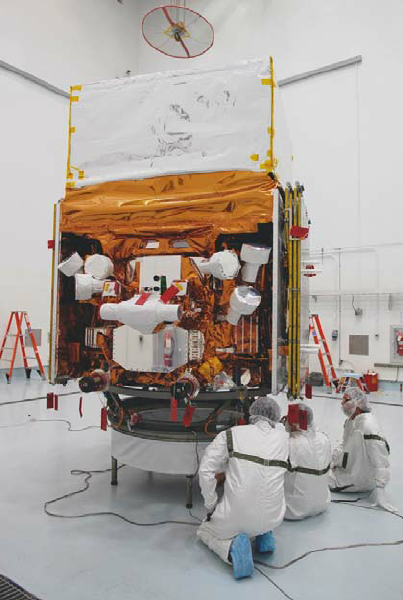
\includegraphics[width=0.5\columnwidth]{figures/fermi2.png}

        % note that in above figure file name, "sr_setup",
        % the file extension is missing. LaTeX is smart enough to find
        % apropriate one (i.e. pdf, png, etc.)
        % You can add this extention yourself as it seen below
        % both notations are correct but above has more flexibility
        %\includegraphics[width=1.0\columnwidth]{sr_setup.pdf}
        \caption{
                \label{fig:fermi} % spaces are big no-no withing labels
                % things like fig: are optional in the label but it helps
                % to orient yourself when you have multiple figures,
                % equations and tables
                The \textit{Fermi} space telescope on Earth, with its solar arrays folded. LAT is the block at the top of the satellite covered with the silver anti-coincidence shield. GBM consists of the cylindrical structures protruding from the lower half of the telescope. Note the size of the engineers relative to the size of the instrument, this highlights the comparatively small effective area of LAT. Image credit: NASA/Kim Shiflett.
        }
\end{figure}

The current workhorse for the majority of space-based $\gamma$-ray observations is the very successful \textit{Fermi} space telescope, which has operated since 2008. \textit{Fermi} is equipped with two instruments, the Large Area Telescope (LAT) which surveys the entire $\gamma$-ray sky every three hours, and the Gamma-Ray Burst Monitor (GBM), which is specifically designed to detect GRBs and solar flares. LAT consists of 18 layers of silicon strip detectors designed to promote pair production from incident $\gamma$-rays, and detect the resultant charged products, as well as a scintillator calorimeter to measure the resultant $\mathrm{e^+/e^-}$ energy (similar in concept to \textit{COS-B}). LAT is able to achieve near perfect background rejection of charged cosmic rays due to the presence of a conducting anti-coincidence shield that surrounds the instrument, such that if a charge signal is detected the instrument will not trigger. GBM consists of two sets of detectors: twelve sodium iodide (NaI) scintillators, and two cylindrical bismuth germanate (BGO) scintillators, and through this can reconstruct the positions of GRBs anywhere on the sky not occluded by the Earth. 

Notable major discoveries by \textit{Fermi} include the detection of the Fermi bubbles, large $\gamma$-ray emitting structures extending to around $\mathrm{20^{\circ}}$ degrees above and below the galactic plane \cite{hooperslayter}, as well as the detection of the short GRB 170817 coincident with a gravitational wave event (GW170817) from a binary neutron star merger \cite{ligogrb}. However, the energy range of LAT is limited to between $\mathrm{20\,MeV}$ and $\mathrm{300\,GeV}$ because of the small effective area of the detector. In order to observe higher-energy photons (in the high GeV-TeV energy range) we must detect them indirectly. This can be performed using the Imaging Atmospheric Cherenkov Telescope (IACT) method, pioneered by Jelly and Galbraith in 1953 \cite{G+J}, and by utilising water Cherenkov detectors  \cite{hawc}. Both of these techniques operate by detecting the Extensive Air Shower (EAS) created when a high energy $\gamma$-ray interacts with Earth's atmosphere. We discuss the specifics of these detectors in the next section. 

\section{Indirect \ensuremath{\gamma}-ray Detection}
\subsection{Historical Instruments}
Jelly and Galbraith \cite{G+J} were the first to create an atmospheric Cherenkov light detector. It consisted of a searchlight mirror, a rubbish bin (painted black on the inside) , an amplifier, an oscilloscope and a single photomultiplier. Following this initial detection, there began a long period of development of the IACT technique (both in terms of instruments and analysis) for astrophysical $\gamma$-ray detection. Early experiments included the 10-meter Whipple telescope in Arizona \cite{whipple}, which is generally considered the first to reliably detect a $\gamma$-ray source from the ground (the Crab Nebula, we will return to the specifics of this detection later in this chapter), as well as the High-Energy-Gamma-Ray Astronomy (HEGRA) experiment on La Palma \cite{HEGRA} and the CANGAROO and Durham telescopes in Australia \cite{CANGAROO} \cite{DURHAM}. Whilst some of the astrophysical detections claimed using these instruments have since been considered controversial \cite{hintonicrc30}, the current era of reliable $\gamma$-ray astronomy from the ground would likely not have been possible without the work performed for these experiments. In the rest of this section we will discuss how current generation IACTs work. 

\subsection{The Cherenkov Effect}
Both IACTs and water Cherenkov detectors ultimately rely upon the Cherenkov effect. Cherenkov light is the light emitted by a medium when a charged particle passes through it faster than the phase velocity of light. An image qualitatively describing the effect can be seen in Figure \ref{fig:jelley}. When a charged particle is at a point P in a dielectric, the atoms surrounding it behave like simple dipoles, with the positive end of the dipole reorienting to point towards the particle if the particle is negatively charged and vice versa. If the particle travels sufficiently slowly, the polarization field surrounding the particle will be completely symmetric, and so when the particle moves on to a new position P', there is no net electric field at a far distance and so no emission. However, if the particle travels faster than the phase velocity of light, whilst the polarization field will still be symmetric along the azimuth, it will no longer be symmetric along the direction of motion. This means that when the system relaxes as the particle moves on a light pulse will be generated \cite{jelley}. As such, as the particle travels through the medium, successive brief pulses of light are generated. 

\begin{figure}[ht] 
        % read manual to see what [ht] means and for other possible options
        \centering 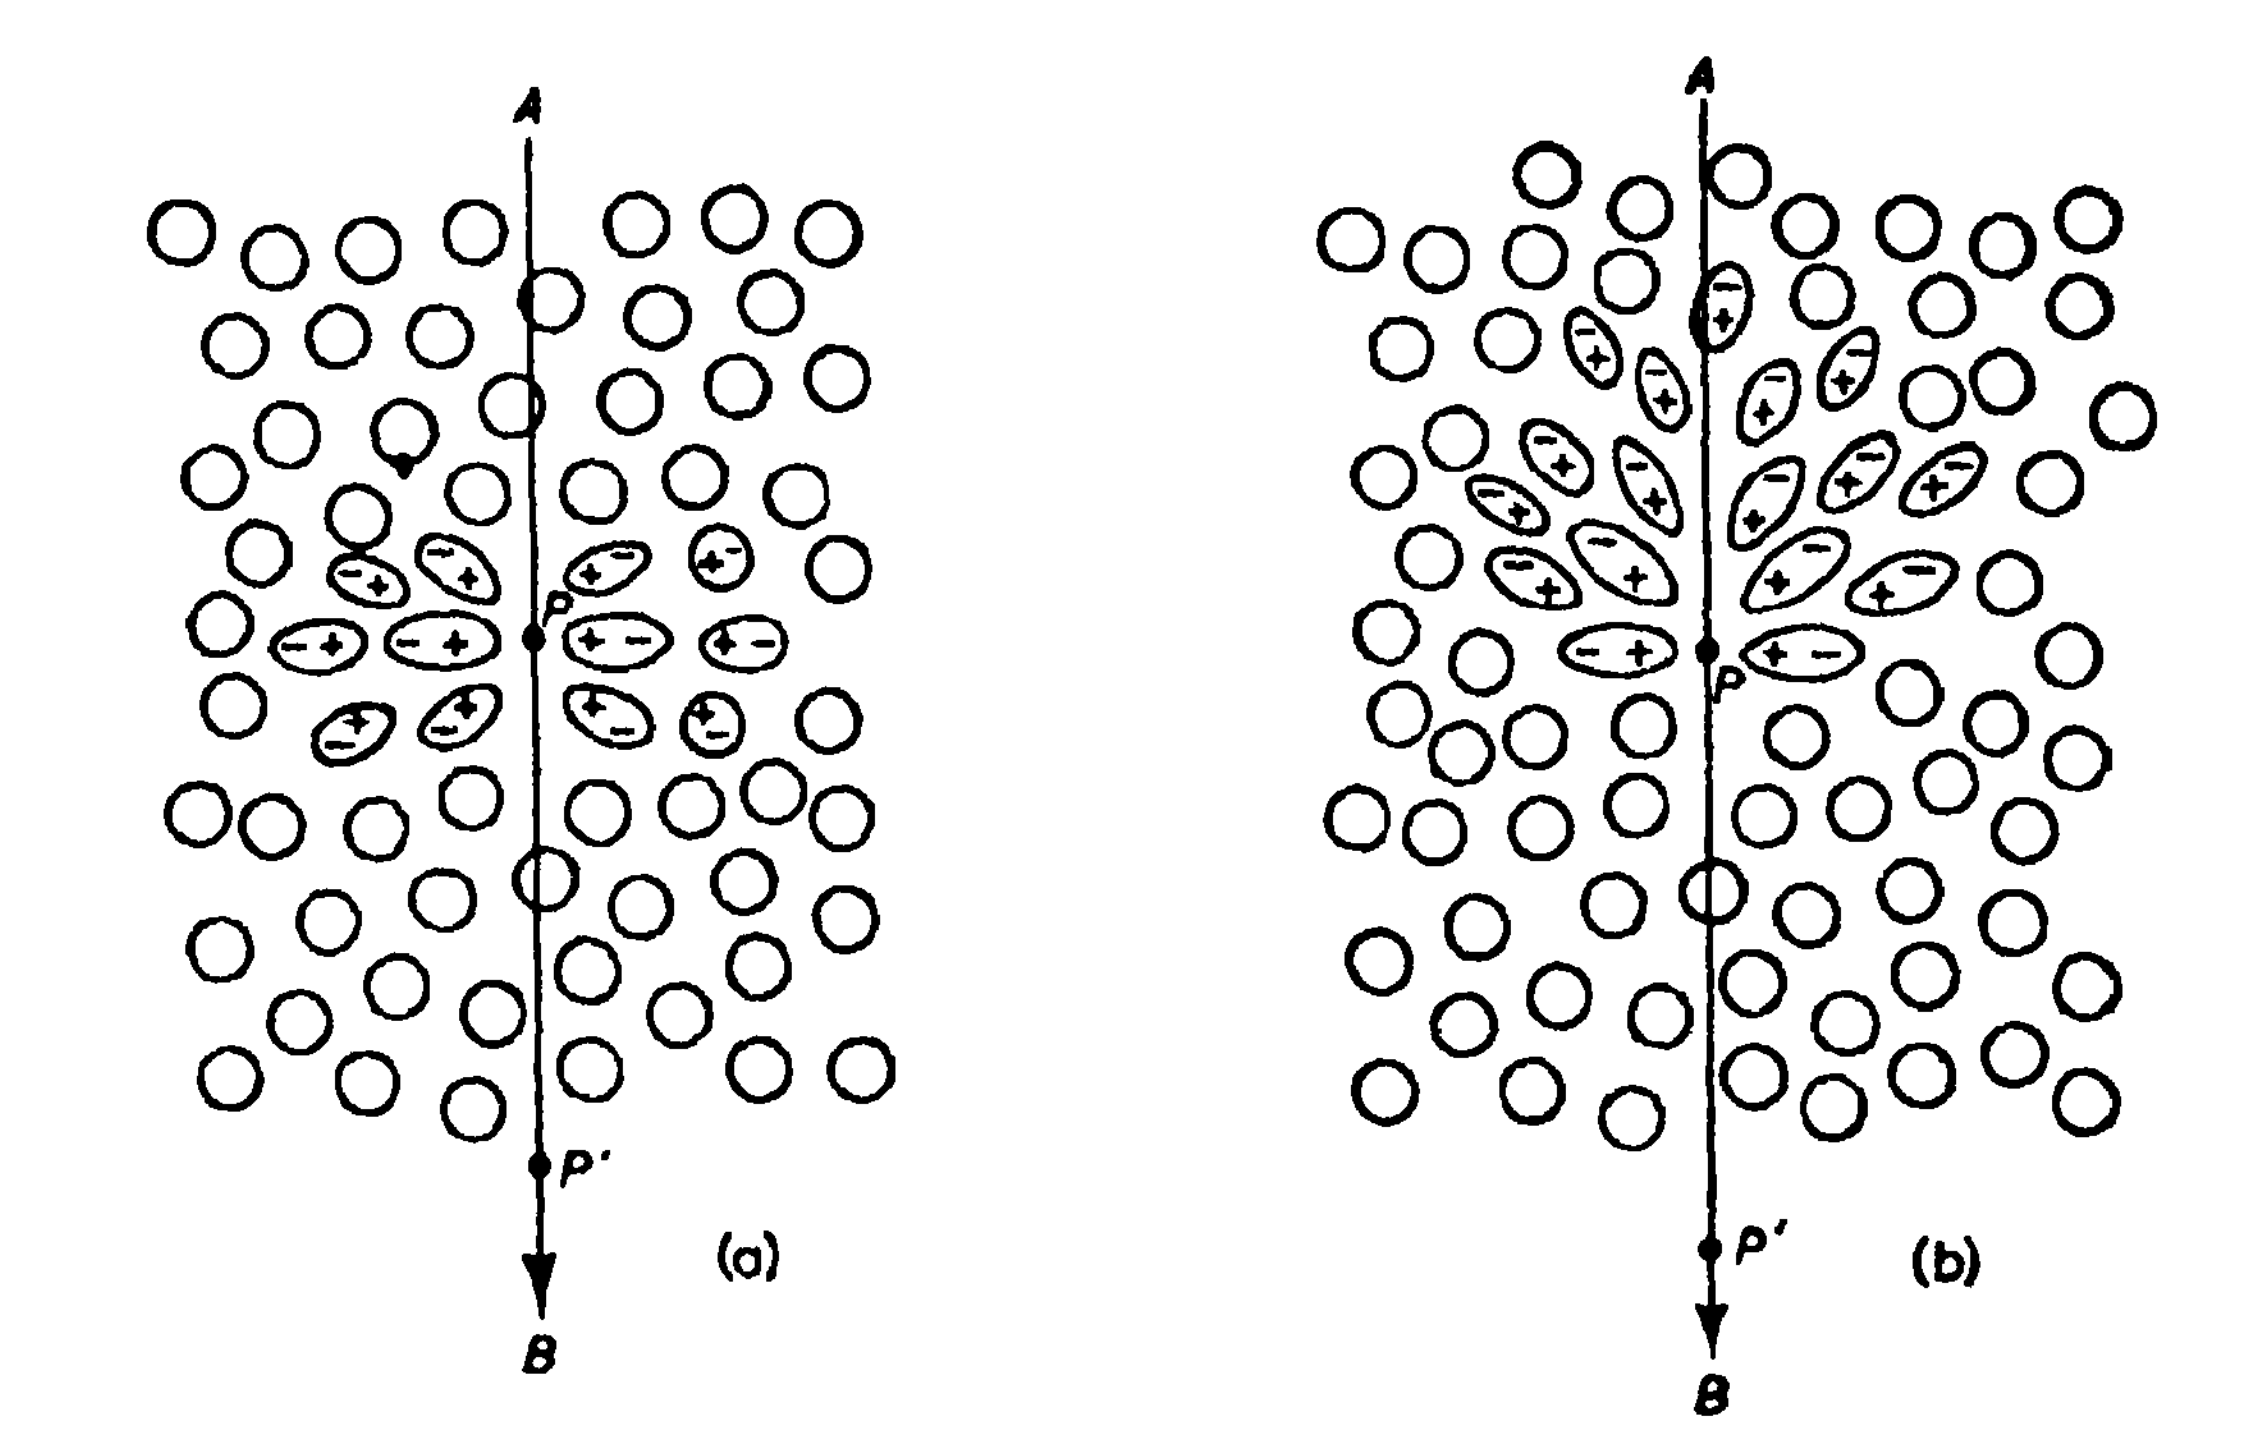
\includegraphics[width=0.7\columnwidth]{figures/dipole.png}

        % note that in above figure file name, "sr_setup",
        % the file extension is missing. LaTeX is smart enough to find
        % apropriate one (i.e. pdf, png, etc.)
        % You can add this extention yourself as it seen below
        % both notations are correct but above has more flexibility
        %\includegraphics[width=1.0\columnwidth]{sr_setup.pdf}
        \caption{
                \label{fig:jelley} % spaces are big no-no withing labels
                % things like fig: are optional in the label but it helps
                % to orient yourself when you have multiple figures,
                % equations and tables
                The polarization set up in a medium by the passage of a charged particle at low velocity (left,a) and high velocity (right,b). Figure taken from \cite{jelley}.
        }
\end{figure}
\begin{figure}[t] 
        % read manual to see what [ht] means and for other possible options
        \centering 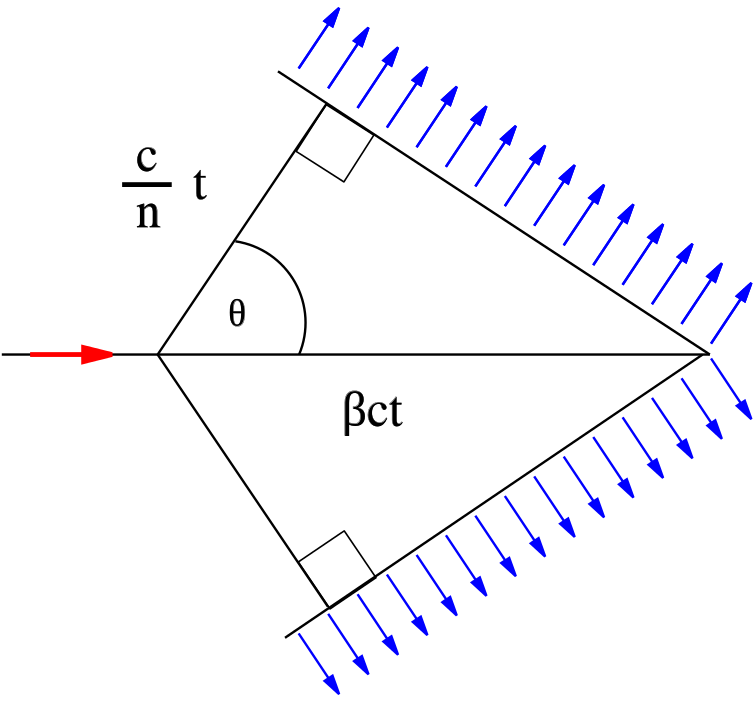
\includegraphics[width=0.5\columnwidth]{figures/Cherenkov.png}

        % note that in above figure file name, "sr_setup",
        % the file extension is missing. LaTeX is smart enough to find
        % apropriate one (i.e. pdf, png, etc.)
        % You can add this extention yourself as it seen below
        % both notations are correct but above has more flexibility
        %\includegraphics[width=1.0\columnwidth]{sr_setup.pdf}
        \caption{
                \label{fig:cherenkov} % spaces are big no-no withing labels
                % things like fig: are optional in the label but it helps
                % to orient yourself when you have multiple figures,
                % equations and tables
                The geometry of the Cherenkov effect, assuming no dispersion. Image credit: A. Horvarth.
        }
\end{figure}

As can be seen in Figure \ref{fig:cherenkov}, this results in the emitted light being distributed according to the Cherenkov opening angle $\theta_c$
\begin{equation}
    \cos\theta_c=\frac{1}{n\beta}
    \label{eq:cherenkov}
\end{equation}

where $n$ is the refractive index, $\beta$=$v/c$ where $v$ is the velocity of light in the medium and $c$ is the speed of light in a vacuum. The energy $dE$ emitted as a result of the particle traversing the medium per unit length $dx$ is given by the Frank-Tamm formula, derived using the framework of special relativity in 1937 (and winning the authors a Nobel prize in 1958 along with Cherenkov). This holds provided the velocity $v$ as a fraction of the speed of light in a vacuum $c$ is greater than $\frac{1}{n(\omega)}$ (where $n(\omega)$ is the frequency dependent refractive index)
\begin{equation}
    \frac{d^2E}{dx\ d\omega}=\frac{q^2}{4\pi}\mu(\omega)\omega\left(1- \frac{c^2}{v^2(\omega)} \right)
    \label{eq:FT}
\end{equation}
where $\mu(\omega)$ is the frequency dependent permeability, and $q$ is the charge of the particle \cite{franktamm}. The total energy emitted in Cherenkov radiation is therefore given by the corresponding integral
\begin{equation}
    \frac{dE}{dx}=\frac{q^2}{4\pi}\int_{v>\frac{c}{n(\omega)}}^{\infty}\mu(\omega)\omega \left(1- \frac{c^2}{v^2n^2(\omega)} \right) d \omega .
    \label{eq:FT2}
\end{equation}

This integral is finite as $\lim_{\omega \to \infty} n(\omega)<1$ and $\lim_{\omega \to 0} n(\omega)=1$ . Assuming $\mu(v)$ is unity equation \ref{eq:FT} can also be integrated over frequency \cite{katz} to get the number of Cherenkov photons $dN_{\gamma}$ emitted per unit length
\begin{equation}
    \frac{dN_{\gamma}}{dx}=2\pi\alpha \left( 1- \frac{1}{\beta^2n^2} \right) \left(\frac{1}{\lambda_{min}}-\frac{1}{\lambda_{max}} \right)
\end{equation}
where $\alpha$ is the fine structure constant, and the $\lambda$ terms represent the minimum and maximum wavelength range of the emission. Taking this band to be $\mathrm{300\,nm-600\,nm}$ and $\beta$=1 implies $\frac{dN_{\gamma}}{dx}$ is around $\mathrm{15\,m^{-1}}$ at an $\mathrm{8\,km}$ altitude in air \cite{katz}. 
\subsection{IACT Basics}

\begin{figure}[ht] 
        % read manual to see what [ht] means and for other possible options
        \centering 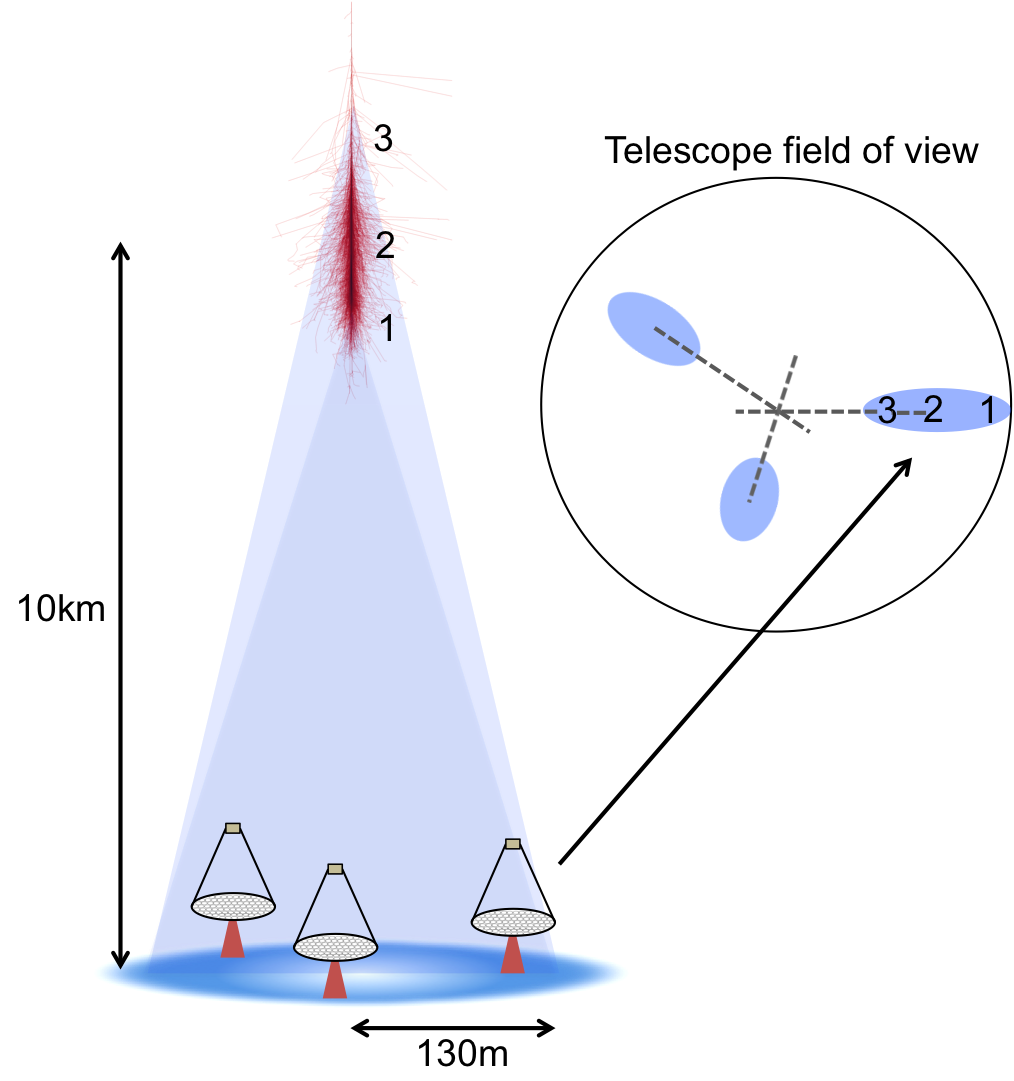
\includegraphics[width=0.7\columnwidth]{figures/schematic.png}

        % note that in above figure file name, "sr_setup",
        % the file extension is missing. LaTeX is smart enough to find
        % apropriate one (i.e. pdf, png, etc.)
        % You can add this extention yourself as it seen below
        % both notations are correct but above has more flexibility
        %\includegraphics[width=1.0\columnwidth]{sr_setup.pdf}
        \caption{
                \label{fig:schem} % spaces are big no-no withing labels
                % things like fig: are optional in the label but it helps
                % to orient yourself when you have multiple figures,
                % equations and tables
                A schematic of the IACT technique, taken from \cite{jamieiact}. Three telescopes stereoscopically observe a
                Cherenkov light pool caused by an EAS. The direction of the incident photon is reconstructed by intersecting the primary axes of 				 the elliptical images in the three cameras. On the right, an illustration that the light from the lowest altitude part of the shower is the first to arrive on the ground.
        }
\end{figure}
When a photon with an energy of above around $\mathrm{20\,GeV}$ encounters the Earth's atmosphere, it undergoes pair production in the electric field of the nucleus of an atmospheric molecule $X$
\begin{equation}
\mathrm{\gamma}+\mathrm{X} \rightarrow \mathrm{X}+\mathrm{e^+}+ \mathrm{e^-}.
\end{equation}
This occurs on average after the $\gamma$-ray travels through one radiation length's worth of atmosphere, typically at around a $\mathrm{20\,km}$ altitude \cite{weekesgamma} (for a more detailed study of the first interaction height of $\gamma$-rays see \cite{Sitarek1i}, it can be estimated using measurements of shower maximum). The resulting electron and positron have very high kinetic energy, and so travel very close to the speed of light in a vacuum and faster than the speed of light in air. As a result, Cherenkov radiation is emitted by the molecules in the vicinity of the particle. The generated particles continue to interact, emitting photons via Brehmsstrahlung radiation, and creating a particle cascade or Extensive Air Shower (EAS). This cascade continues down into the atmosphere until the radiation and ionisation losses become equal, which is also the point at which the maximum number of particles ($N_{Max}$) are present in the shower as a function of atmospheric mass traversed (in $\mathrm{g\,cm^{-2}}$). This point is known as the shower maximum (denoted $X_{Max}$). The altitude at which this occurs is referred to as $h_{Max}$, after which point the energy losses dominate and the number of produced particles significantly reduces. For an incident $\gamma$-ray of $\mathrm{10\,TeV}$ energy, $X_{Max}\approx \mathrm{431\,g\,cm^{-2}}$, $h_{Max}=\mathrm{6.8\,km}$ and $N_{Max}=\mathrm{1.0 \times 10^4}$ \cite{weekesgamma}.  The Cherenkov light produced from this EAS forms a pool on the ground of radius $\sim\mathrm{120\,m}$ \cite{weekesgamma}, and this can be observed with an optical frequency telescope on the ground at night provided it is equipped with an extremely fast (ns timescale) camera, as the Cherenkov light flash from an 
EAS is of the order of a few ns. 

In order to optimally reconstruct the energy and direction of the incident $\gamma$-ray, data from an array of such telescopes is typically combined stereoscopically, a technique pioneered by the HEGRA instrument in the 1990s \cite{HEGRA}. This use of stereoscopy improves background rejection power as the chances of directly imaging a muon ring originating from a proton shower are higher, and with multiple images the determination of shower width is more accurate.  The optimal spacing for these telescopes is of the same order as the size of the light pool on the ground \cite{weekesgamma}.

Given that the only (not heavily-suppressed) interactions possible in an $\gamma$-ray or electron induced air shower are pair production and $\gamma$-ray brehmstrahlung, it is possible to construct a simple model of their evolution (the Heitler model) \cite{heitler}. Given that the radiation length of an electron in the atmosphere is known to be $X_0=\mathrm{36.7\,g\,cm^{-2}}$, the typical length over which a new pair production will occur is $N_0=X_0 \ln 2$. After $n$ interactions the atmospheric grammage traversed is $x=nX_0 \ln 2$, and the number of surviving particles is $N=2^n=\exp \left( \frac{x}{X_0}\right)$. Assuming the particle energies are uniformly distributed, the energy per particle $E=E_0/N$ (where $E_0$ is the initial energy of the originally incident particle. Given that the shower maximum occurs when $E=E_c^e=\mathrm{85\,MeV}$, the number of particles at $X_{Max}$ is given by 
\begin{equation}
    N_{Max}=2^{n_c}=\frac{E_0}{E_c^e}
\end{equation}
where $n_c=\frac{\ln (\frac{E_0}{E_e^c})}{\ln 2}$ \cite{heitler}.

\section{Current Generation Indirect Detection Instruments}
\subsection{VERITAS}
Very Energetic Radiation Imaging Telescope Array System (VERITAS) consists of four 12-meter parabolic, single mirror IACTs at the Fred Lawrence Whipple Observatory in Arizona (the original VERITAS design intended eight IACTs). Construction of VERITAS began in 2003 and was completed in 2007. It is designed to give optimal sensitivity in the $\mathrm{100\,GeV}$ to $\mathrm{10\,TeV}$ energy band. Recent work performed by VERITAS includes the discovery of a flare in the gamma-ray emission from the Blazar TXS 0506+056, coincident in space and time with a neutrino detection from IceCube \cite{TXS}, and the detection of TeV gamma-rays from the redshift 0.939 Blazar PKS 1441+25, indicating the transparency of the universe to photons of such energies \cite{escape}. In Chapter \ref{ch:4-VERITASRealData}, we use real observations from VERITAS to test deep-learning-based event classification as a technique intended for use by the next generation Cherenkov Telescope Array (CTA).

\subsection{MAGIC}
Major Atmospheric Gamma Imaging Cherenkov Telescopes (MAGIC) consists of two 17-meter-diameter IACTs on La Palma, designed to detect $\gamma$-rays with energies between $\mathrm{25\,GeV}$ and $\mathrm{30\,TeV}$. MAGIC's cameras are unusual as they consist of two separate types of conventional photomultiplier, 386 hexagonal pixels in the centre surrounded by 180 larger pixels at the edge. A major aim of MAGIC was to hunt for Gamma-Ray Bursts (GRBs) from the ground, a goal it achieved when it detected TeV $\gamma$-rays from GRB 190114C in early 2019 \cite{magicGRB} (H.E.S.S. CT5 also detected the subsequent afterglow).

\subsection{H.E.S.S.}
The High Energy Stereoscopic System (H.E.S.S.) is an IACT array in the Khomas Highlands of Namibia. H.E.S.S. is the only current generation instrument to consist of multiple classes of IACT, four with a $\sim$12-meter-diameter mirror (CT1-4) and a fifth (CT5) with a 28-meter-diameter mirror, giving it an operational energy range of $\mathrm{30\,GeV}$ to $\mathrm{100\,TeV}$. Construction of the four original $\mathrm{12\,m}$ instruments was completed in 2003, with the larger telescope completed in 2012. The H.E.S.S. cameras have been upgraded twice. In 2015 the CT1-4 telescopes were upgraded with improved ventilation and NECTAr-based front-end electronics \cite{hess1u}. Then in 2019 CT5 was upgraded with a new fully-digitized trigger and readout system and higher-efficiency photomultipliers. Notable recent achievements of H.E.S.S. include resolving the extension of the Crab Nebula \cite{crabextension} and the jet of Centaurus A \cite{cena} for the first time (with an IACT).

\subsection{FACT}
The First G-APD Cherenkov Telescope (FACT) is an autonomous upgrade of a former HEGRA Cherenkov telescope, notable for being the first instrument to attempt the use of Silicon Photomultipliers (SiPMs) in Cherenkov astronomy. Given it is a single IACT and not an array, however, its sensitivity is limited. As such it largely operates as a blazar monitoring instrument, such that other instruments can be notified in the event of a flare. 

FACT arguably has one of the most advanced analysis chains of the current IACTs, which is largely based in Python, and this has had a partial influence on CTA's analysis chain. Notably the FACT collaboration used open source, Python-based analysis tools developed using modern version control (with git and github) \cite{factspec}. This was not the case for any of the other analysis chains developed for the other current IACTs which remain largely based on root.

\subsection{HAWC, Tibet AS-\ensuremath{\gamma} and LHASSO}

The IACT technique is not the only means of indirect $\gamma$-ray detection from the ground. At sufficiently high altitude, one can use Water Cherenkov detectors to directly observe the electrons from an incident shower, and then use arrival time information as a background rejection method. This is the key principle underlying the successful High Altitude Water Cherenkov (HAWC) observatory in Mexico \cite{hawc}, as well the principle behind the Chinese Tibet AS-$\gamma$ \cite{asgamma} and Large High Altitude Air Shower Observatory (LHASSO) \cite{lhassocrab} experiments (the currently under construction LHASSO detector will also have small IACTs on site). These complement IACTs with their main advantage of being that these are survey instruments with a wide field of view, higher operational energy range and nearly $100\%$ duty cycle (for IACTs this is closer to $10\%$, but comparatively poor angular resolution and background rejection. 

\section{The Cherenkov Telescope Array and Associated Instruments}
\subsection{Concept}
The Cherenkov Telescope Array (CTA) is an ambitious project to build a next-generation VHE $\gamma$-ray facility, which aims to improve on the sensitivity of the current generation instruments by roughly an order of magnitude \cite{scienceCTA}. The CTA consortium, involved in directing CTA Observatory (CTAO) science goals and array design, consists of over 1400 scientists from 31 countries around the globe. Given the large energy range ($\mathrm{20\,GeV}$ to $\mathrm{300\,TeV}$) that CTA will operate  over \cite{scienceCTA}, three classes of IACT are required. These are designated as the Small-, Medium- and Large-Sized Telescopes (SSTs, MSTs and LSTs). The 23-meter-diameter LSTs are designed for high sensitivity observations of $\gamma$-rays over the $\mathrm{20\,GeV}$ to $\mathrm{150\,GeV}$ energy range, increasing the overlap in sensitivity with space-based missions such as the \textit{Fermi} $\gamma$-ray Space Telescope \cite{Fermi}. The SSTs will be the smallest (approximately 4-meter-diameter) but most numerous telescopes, and will be spread out over a large ($\sim$4 km$^2$) area in order to maximise CTA's effective area for $\gamma$-ray energies over $\mathrm{5\,TeV}$. The MSTs will provide unprecedented sensitivity to cosmic $\gamma$-ray fluxes in the intermediate energy range. The baseline (`omega' configuration) design of CTA consists of 99 telescopes (4 LSTs, 25 MSTs, 70 SSTs) placed on a southern site at Cerro Paranal in Chile, whereas a smaller array of 19 telescopes (4 LSTs, 15 MSTs, and no SSTs) will be placed on a northern site on Spanish Canary Island of La Palma. By having both a northern and southern site, the CTA Observatory will cover the whole sky \cite{scienceCTA}. However, as of writing this thesis, the current construction plan for CTA is to first build a so-called `alpha' configuration array consisting of 4 LSTs and 9 MSTs in the northern site, and 14 MSTs and 37 SSTs in the southern array. Further details regarding the science performance of the SST sub-array and the complete CTA instrument can be found in Maier et. al \cite{gernotCTA} and Hassan et. al \cite{tarekCTA}.
\begin{figure}[ht!] 
        % read manual to see what [ht] means and for other possible options
        \centering 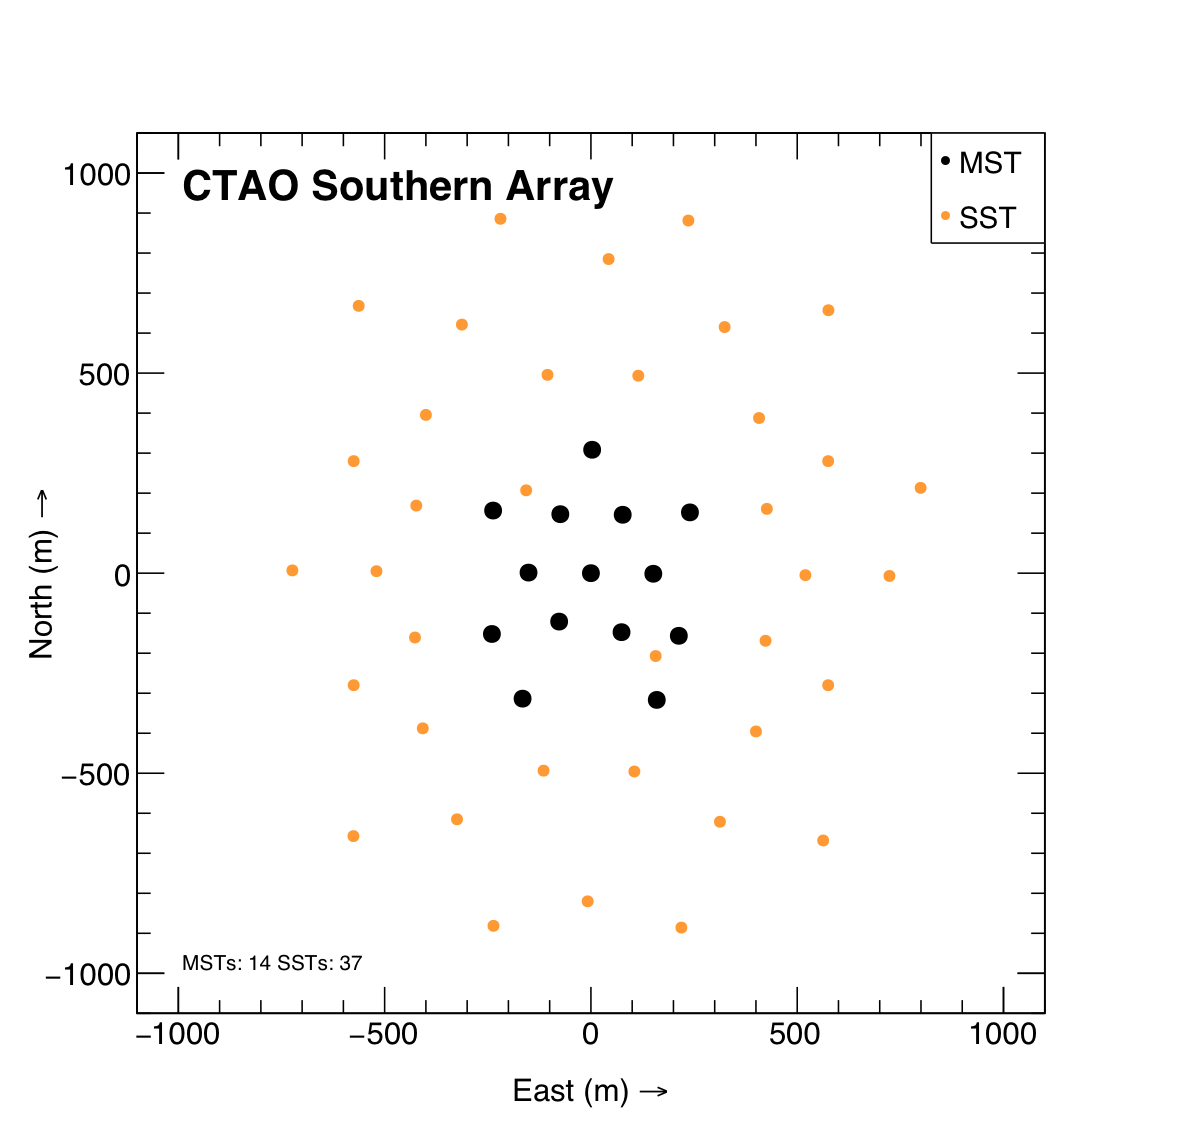
\includegraphics[width=0.7\columnwidth]{figures/southlayout.png}
        % note that in above figure file name, "sr_setup",
        % the file extension is missing. LaTeX is smart enough to find
        % apropriate one (i.e. pdf, png, etc.)
        % You can add this extention yourself as it seen below
        % both notations are correct but above has more flexibility
        %\includegraphics[width=1.0\columnwidth]{sr_setup.pdf}
        \caption{
                \label{fig:southlayout} % spaces are big no-no withing labels
                % things like fig: are optional in the label but it helps
                % to orient yourself when you have multiple figures,
                % equations and tables
                The CTA-South alpha array configuration, taken from \cite{zencta}.
        }
\end{figure}
\subsection{CHEC and SSTCAM}
\begin{figure}[ht] 
        % read manual to see what [ht] means and for other possible options
        \centering 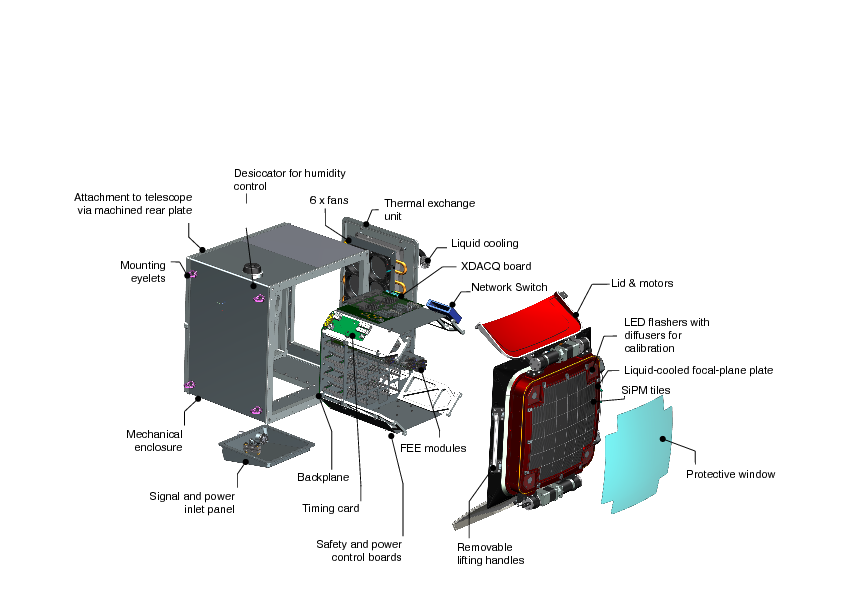
\includegraphics[width=\columnwidth]{figures/cam.png}
        % note that in above figure file name, "sr_setup",
        % the file extension is missing. LaTeX is smart enough to find
        % apropriate one (i.e. pdf, png, etc.)
        % You can add this extention yourself as it seen below
        % both notations are correct but above has more flexibility
        %\includegraphics[width=1.0\columnwidth]{sr_setup.pdf}
        \caption{
                \label{fig:cam} % spaces are big no-no withing labels
                % things like fig: are optional in the label but it helps
                % to orient yourself when you have multiple figures,
                % equations and tables
                The CHEC-S Computer Aided Design (CAD) model with key elements highlighted, taken from \cite{rwhite}.
        }
\end{figure}
The UK's main material contribution to CTA construction is planned to be construction of SST Cameras (SSTCAMs). These are an upgraded version of the earlier Compact High Energy Camera (CHEC) prototypes, which were designed to work with SST structures that have a dual-mirror (Swartzchild-Couder) optical design. This design allows for a compact camera (approximately 0.4-meter-diameter) with small scale photosensors ($\mathrm{6/7\,mm}$, corresponding to roughly a third of the plate scale of a comparable single-mirror design) and a wide field of view ($\mathrm{\sim0.2\,^{\circ}/pixel}$).  Two operational CHEC prototypes have already been built. The first, CHEC-M, has as its light detectors 32 Multi-Anode Photomultipliers (MAPMs) \cite{tomthesis}. These consist of a block of 8x8 pixels, the signals from which are digitised at a rate of $1\mathrm{GSa}/\mathrm{s}$ \cite{tomthesis} by front end electronics based upon the custom TARGET Application-Specific Integrated Circuit (ASIC) \cite{checmpaper}. These blocks of front end electronics per photomultiplier tile are known as a TARGET Module (TM). When the camera is triggered by two or more four pixel blocks (superpixels) exceeding a discriminator threshold, the data is read out of the `fast chain' of the camera over a configurable window in blocks of 32 samples (roughly corresponding to a nanosecond each). CHEC simultaneously has a slow-signal chain with a longer integration window in order to detect stars for pointing calibration. A refined prototype, CHEC-S, is currently undergoing testing at the Max Planck Institute for Nuclear Physics in Heidelberg. CHEC-S contains a refinement of the TARGET-based electronics of its predecessor, but replaces the MAPMs with SiPMs. These have the advantage of being more physically durable and easier to operate than MAPMs (not requiring a high-voltage supply), as well as having a less notable drop in Photon Detection Efficiency (PDE) over time \cite{factphotonstream}. Crucially SiPMs can also operate in conditions with a higher Night Sky Background (NSB) compared to MAPMs, allowing for routine observations under partial moonlight with little degradation in performance. CHEC-S also added a curved front window that helps to attenuate NSB whilst transmitting Cherenkov light \cite{ssticrc}. A final prototype SSTCAM engineering camera (with a new, easier to fabricate flat window) is currently undergoing construction, and will be the first SST camera delivered to CTAO.

Both CHEC cameras and the SSTCAM engineering camera have self-calibration LED flasher systems, designed to flat-field the camera. The flashers on the CHEC prototypes were attached to the camera corners and reflected off the secondary mirror of the dual-mirror telescope it is attached to, for the final SST Camera (SSTCAM) design the flasher will most likely be situated behind the secondary mirror and shine through.

\subsection{GCT, ASTRI and the SST Harmonization Process}

There are two SST dual-mirror prototype SST designs that CHEC cameras can be attached to, the French led \textit{Gamma Cherenkov Telescope} (GCT), and the Italian led \textit{Astrofisica con Specchi a Tecnologia Replicante Italiana} (ASTRI) instrument. Both share the same Schwarzchild-Couder optical design, which allows for a compact SiPM camera as well as a more uniform Point Spread Function (PSF) across the Field of View (FoV). Following a harmonisation process, the ASTRI telescope structure with a CHEC-type camera was selected as the basis for the final SST design, taking into account lessons learned from all prototypes. As a result, the CHEC collaboration changed its name to the SSTCAM collaboration. But for the results in this thesis (which are primarily concerned with the camera), these two optical structures are largely interchangeable (in Chapter \ref{ch:3-TimingInfo} we consider CHEC-S with GCT as our instrument, whereas in Chapter \ref{ch:5-CHECNSB} we consider CHEC-S on ASTRI). We also consider CHEC-S to be broadly representative of the final SSTCAM, as the pixel sizes and configurations (the biggest influence upon our analysis) will likely be very similar.

\begin{figure}[ht] 
        % read manual to see what [ht] means and for other possible options
        \centering 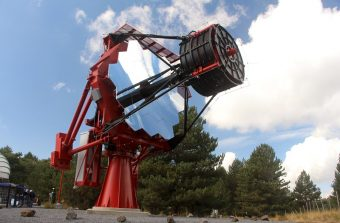
\includegraphics[width=\columnwidth]{figures/astri-horn.jpg}
        % note that in above figure file name, "sr_setup",
        % the file extension is missing. LaTeX is smart enough to find
        % apropriate one (i.e. pdf, png, etc.)
        % You can add this extention yourself as it seen below
        % both notations are correct but above has more flexibility
        %\includegraphics[width=1.0\columnwidth]{sr_setup.pdf}
        \caption{
                \label{fig:astri} % spaces are big no-no withing labels
                % things like fig: are optional in the label but it helps
                % to orient yourself when you have multiple figures,
                % equations and tables
                The ASTRI-Horn prototype on Sicily. Image Credit: CTA Collaboration.
        }
\end{figure}

\section{Types of IACT Backgrounds}
\subsection{Hadronic Air Showers}

In order to perform IACT $\gamma$-ray observations, we need to be able to distinguish astrophysical $\gamma$-ray signals from background reliably. At most energies, EAS caused by incident charged hadrons (most commonly protons) outnumber those caused by photons by a factor of roughly 10,000 \cite{Benbow}. These provide a significant background to IACTs, and are the largest constraint on their sensitivity, as at IACT energies charged cosmic rays (protons, electrons and heavier nuclei) cannot be traced back to their origin due to scattering in the galactic magnetic field.

\begin{figure}
\begin{center}  

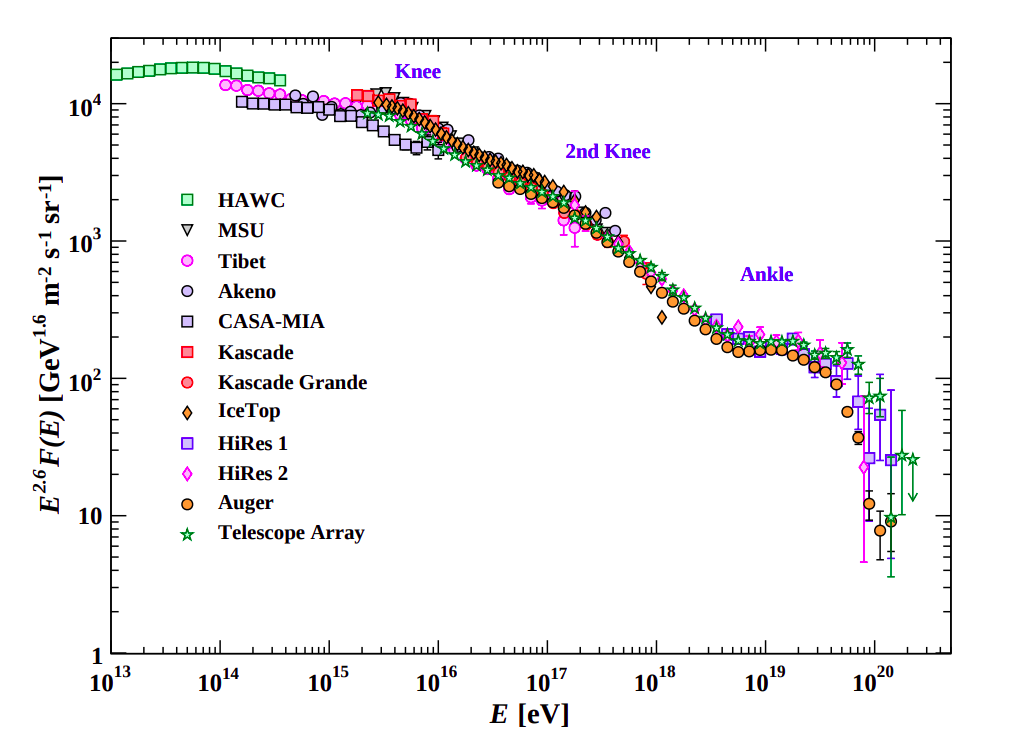
\includegraphics[width=\columnwidth]{figures/pdgcr.png}
 
\caption{The all particle cosmic ray spectrum, taken from \cite{pdg}. Whilst mainly protons, this spectrum includes both cosmic ray electrons and heavier element cosmic rays. The spectrum is a power law with index $\mathrm{-2.7}$ up to around $\mathrm{3 \times 10^6\,GeV}$, where it steepens to an index of $\mathrm{-3.1}$, a transition feature known as `the knee'. It then flattens back to an index of -2.7 at $\mathrm{4 \times 10^9\,GeV}$ (a feature known as `the ankle'. The lower energy cosmic rays below the knee are believed to be galactic in origin, most likely a result of acceleration in supernova remnants. The higher energy cosmic rays above the knee are believed to be the result of cosmic ray acceleration in extragalactic sources such as AGN. The so-called GZK cutoff is theorised to exist at energies around $\mathrm{50\,EeV}$ \cite{gzk}, the limit at which a cosmic ray could propagate from another galaxy without interacting with the CMB. For comparison, the Large Hadron Collider operates at a centre of mass energy of $\mathrm{14\,TeV}$ for proton-proton collisions, corresponding to an initial EAS proton energy of $\mathrm{1\times 10^{17}\,eV}$.}
\label{fig:crspec}
\end{center}
\end{figure}

However, because the quarks contained within protons experience the strong nuclear force, the   interactions hadrons undergo on entering the atmosphere are different to photons. When these charged hadrons collide with atmospheric nuclei, a typical interaction scheme between the two protons \cite{EAS} is
\begin{gather*}
\mathrm{p}+\mathrm{p}\rightarrow \mathrm{N}+\mathrm{N}+n_1 (\mathrm{\pi^+ + \pi^- })+n_2\mathrm{\pi^0} \\
\mathrm{\pi^0} \rightarrow \mathrm{2\gamma} \\
\mathrm{\mathrm{\pi^{\pm}}} \rightarrow \mathrm{\mu^{\pm}}+\mathrm{\overset{(-)}{\nu_{\mu}}}\\
\mathrm{\mu^{\pm}} \rightarrow \mathrm{e^{\pm}}+\mathrm{\overset{(-)}{\nu_{\mu}}}+\mathrm{\overset{(-)}{\nu_{e}}}
\end{gather*}
where $N$ represents the resulting fragmented hadrons which are produced along with $n_1$ charged pions and $n_2$ neutral pions. The charged pions have a short lifetime of only $\mathrm{26\,ns}$, but the neutral pions' lifetime is even shorter at $5 \times 10^{-17}\,\mathrm{s}$ because they decay to two photons via the electromagnetic force. Kaon production is also possible in hadronic EAS at higher energies, though the resultant products are the same. Despite their short lifetime, as the charged muons produced in EAS are highly relativistic some can survive to ground level as a result of time dilation effects. The other charged muons decay to electrons, positrons and neutrinos via the weak nuclear force. In a hadronic EAS muons undergo a significant number of inelastic scattering interactions, carrying a larger fraction of the total transverse momentum away from the shower core and resulting in a wider overall EAS for proton showers compared to a $\gamma$-ray induced shower \cite{tomthesis}.  The resultant $\gamma$-rays from $\pi_0$ decay can themselves undergo pair production creating electromagnetic sub-showers of the hadronic shower core. Similarly to $\gamma$-ray EAS, as the charged products from all of these interactions are typically highly relativistic they produce detectable Cherenkov light. But these physical differences in the interactions between $\gamma$-ray and hadronic EAS are the basis for the background rejection techniques we'll encounter later in this chapter. Whilst the interaction scheme for hadronic air showers is more complex than for $\gamma$-ray or electron induced ones, it is still possible to construct semi-analytic models of their evolution. The most notable of these is the Heitler-Matthew model, details regarding this can be found in \cite{heitler}. As we'll see later in this chapter, similar hadronic interactions can occur in astrophysical environments.
\begin{figure}[h!]
\begin{center}  

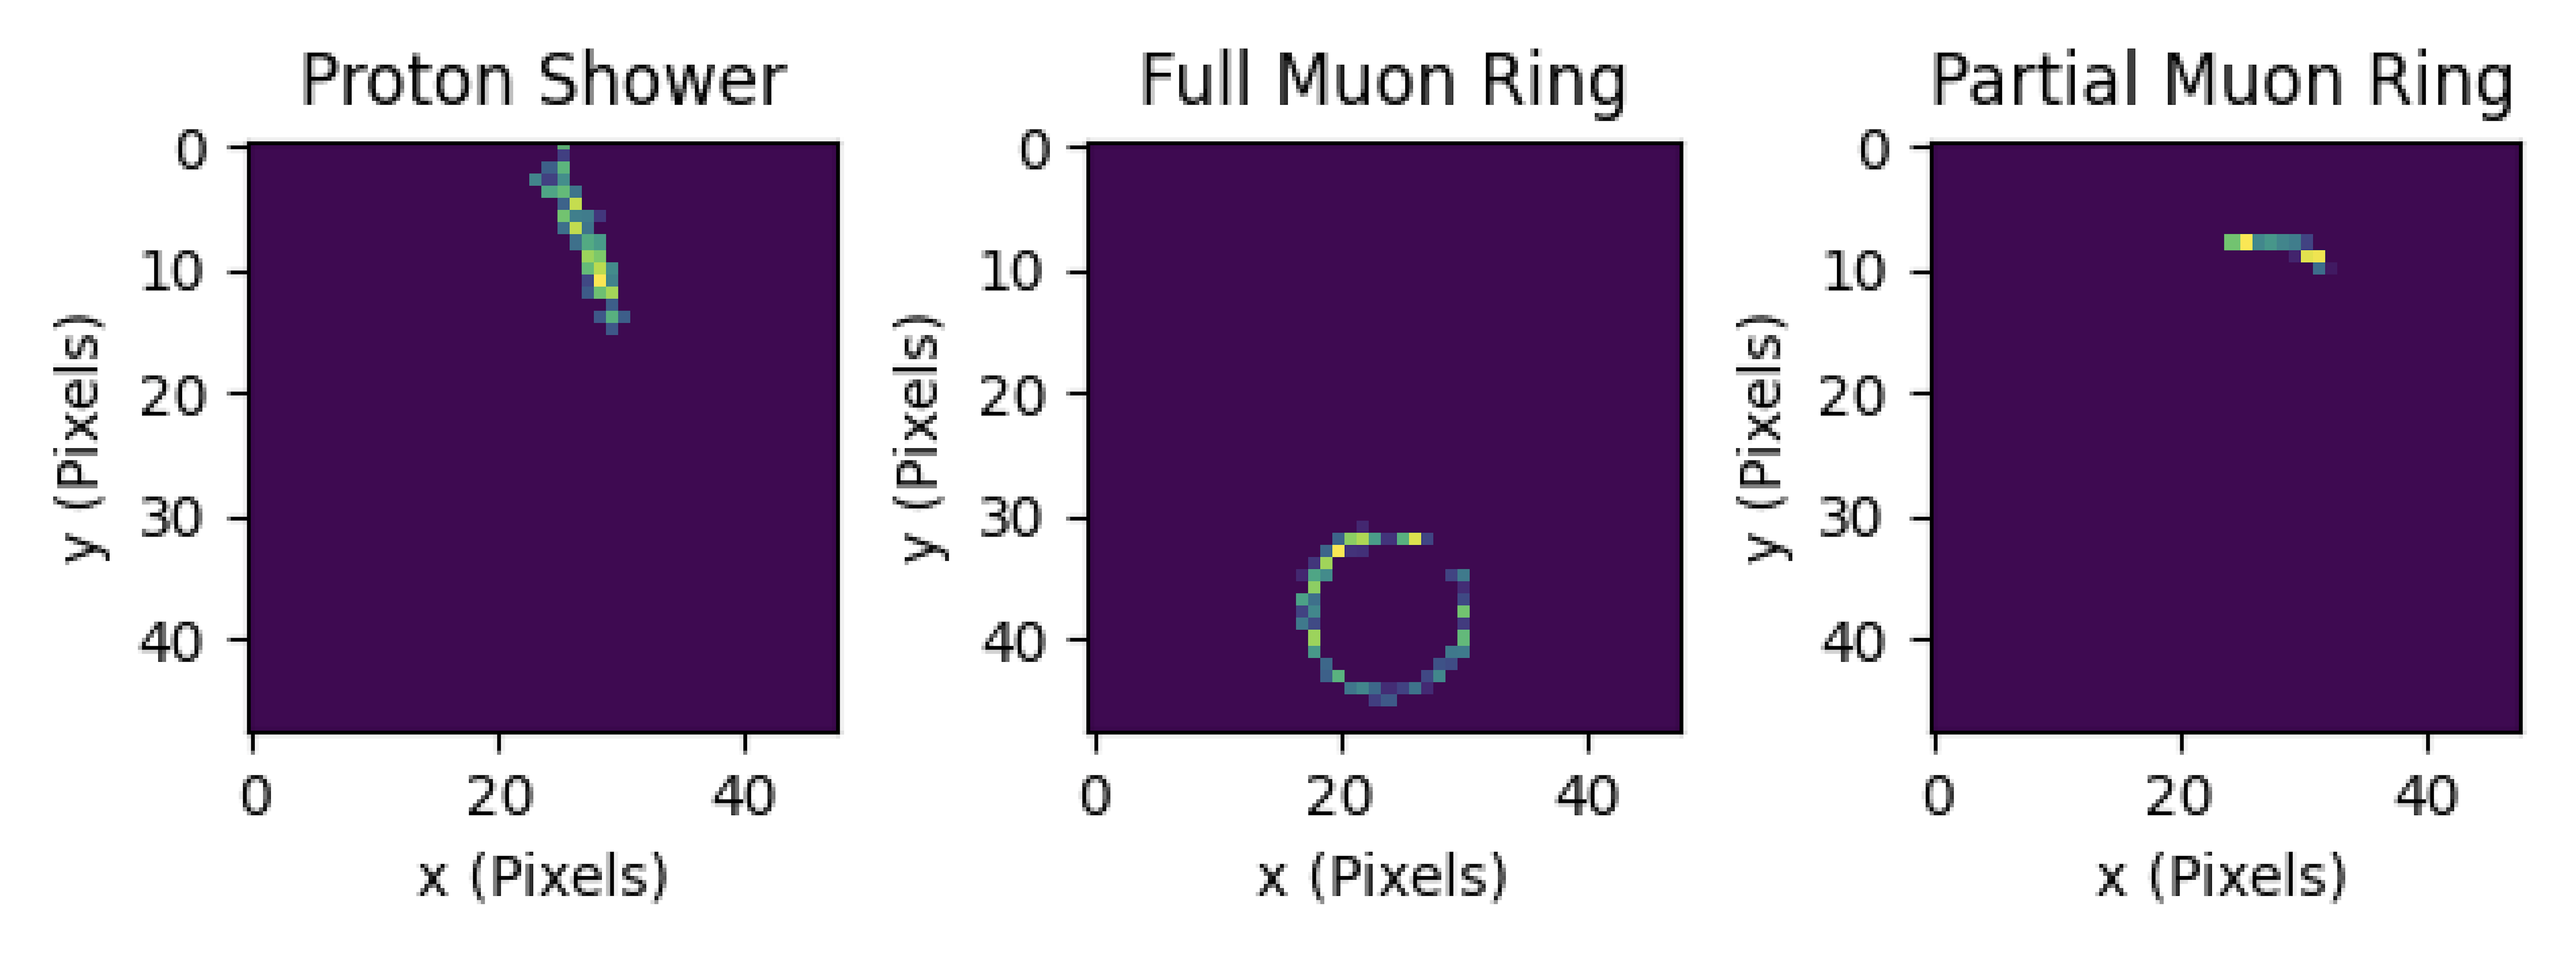
\includegraphics[width=\columnwidth]{figures/muonplot.png}
 
\caption{A proton shower image, a full muon ring image, and a partial muon ring image. These were generated using \textit{CORSIKA}/\textit{sim\_telarray} simulations of CHEC-S on ASTRI. The partial muon ring effect was generated by changing the impact distance from the telescope using the \textit{CORSIKA} CSCAT parameter.}
\label{fig:muonplot}
\end{center}
\end{figure}

Muons that survive to ground level and that pass directly along the optical axis of the telescope create characteristic Cherenkov `ring' images in the camera. These muon rings are useful for online calibration as the width of the muon ring image is proportional to the incident particle energy. The observed pixel intensity can then be compared to the expected intensity for a muon with that energy and can thus be used to compute the optical efficiency of the telescope system. Muons that pass off-axis to the telescope are only partially imaged; at sufficiently large impact parameters these partial muon ring images can closely resemble those of $\gamma$-ray EAS, creating an additional source of background. An example of such images can be seen in Figure \ref{fig:muonplot}.

\begin{figure}
\begin{center}  

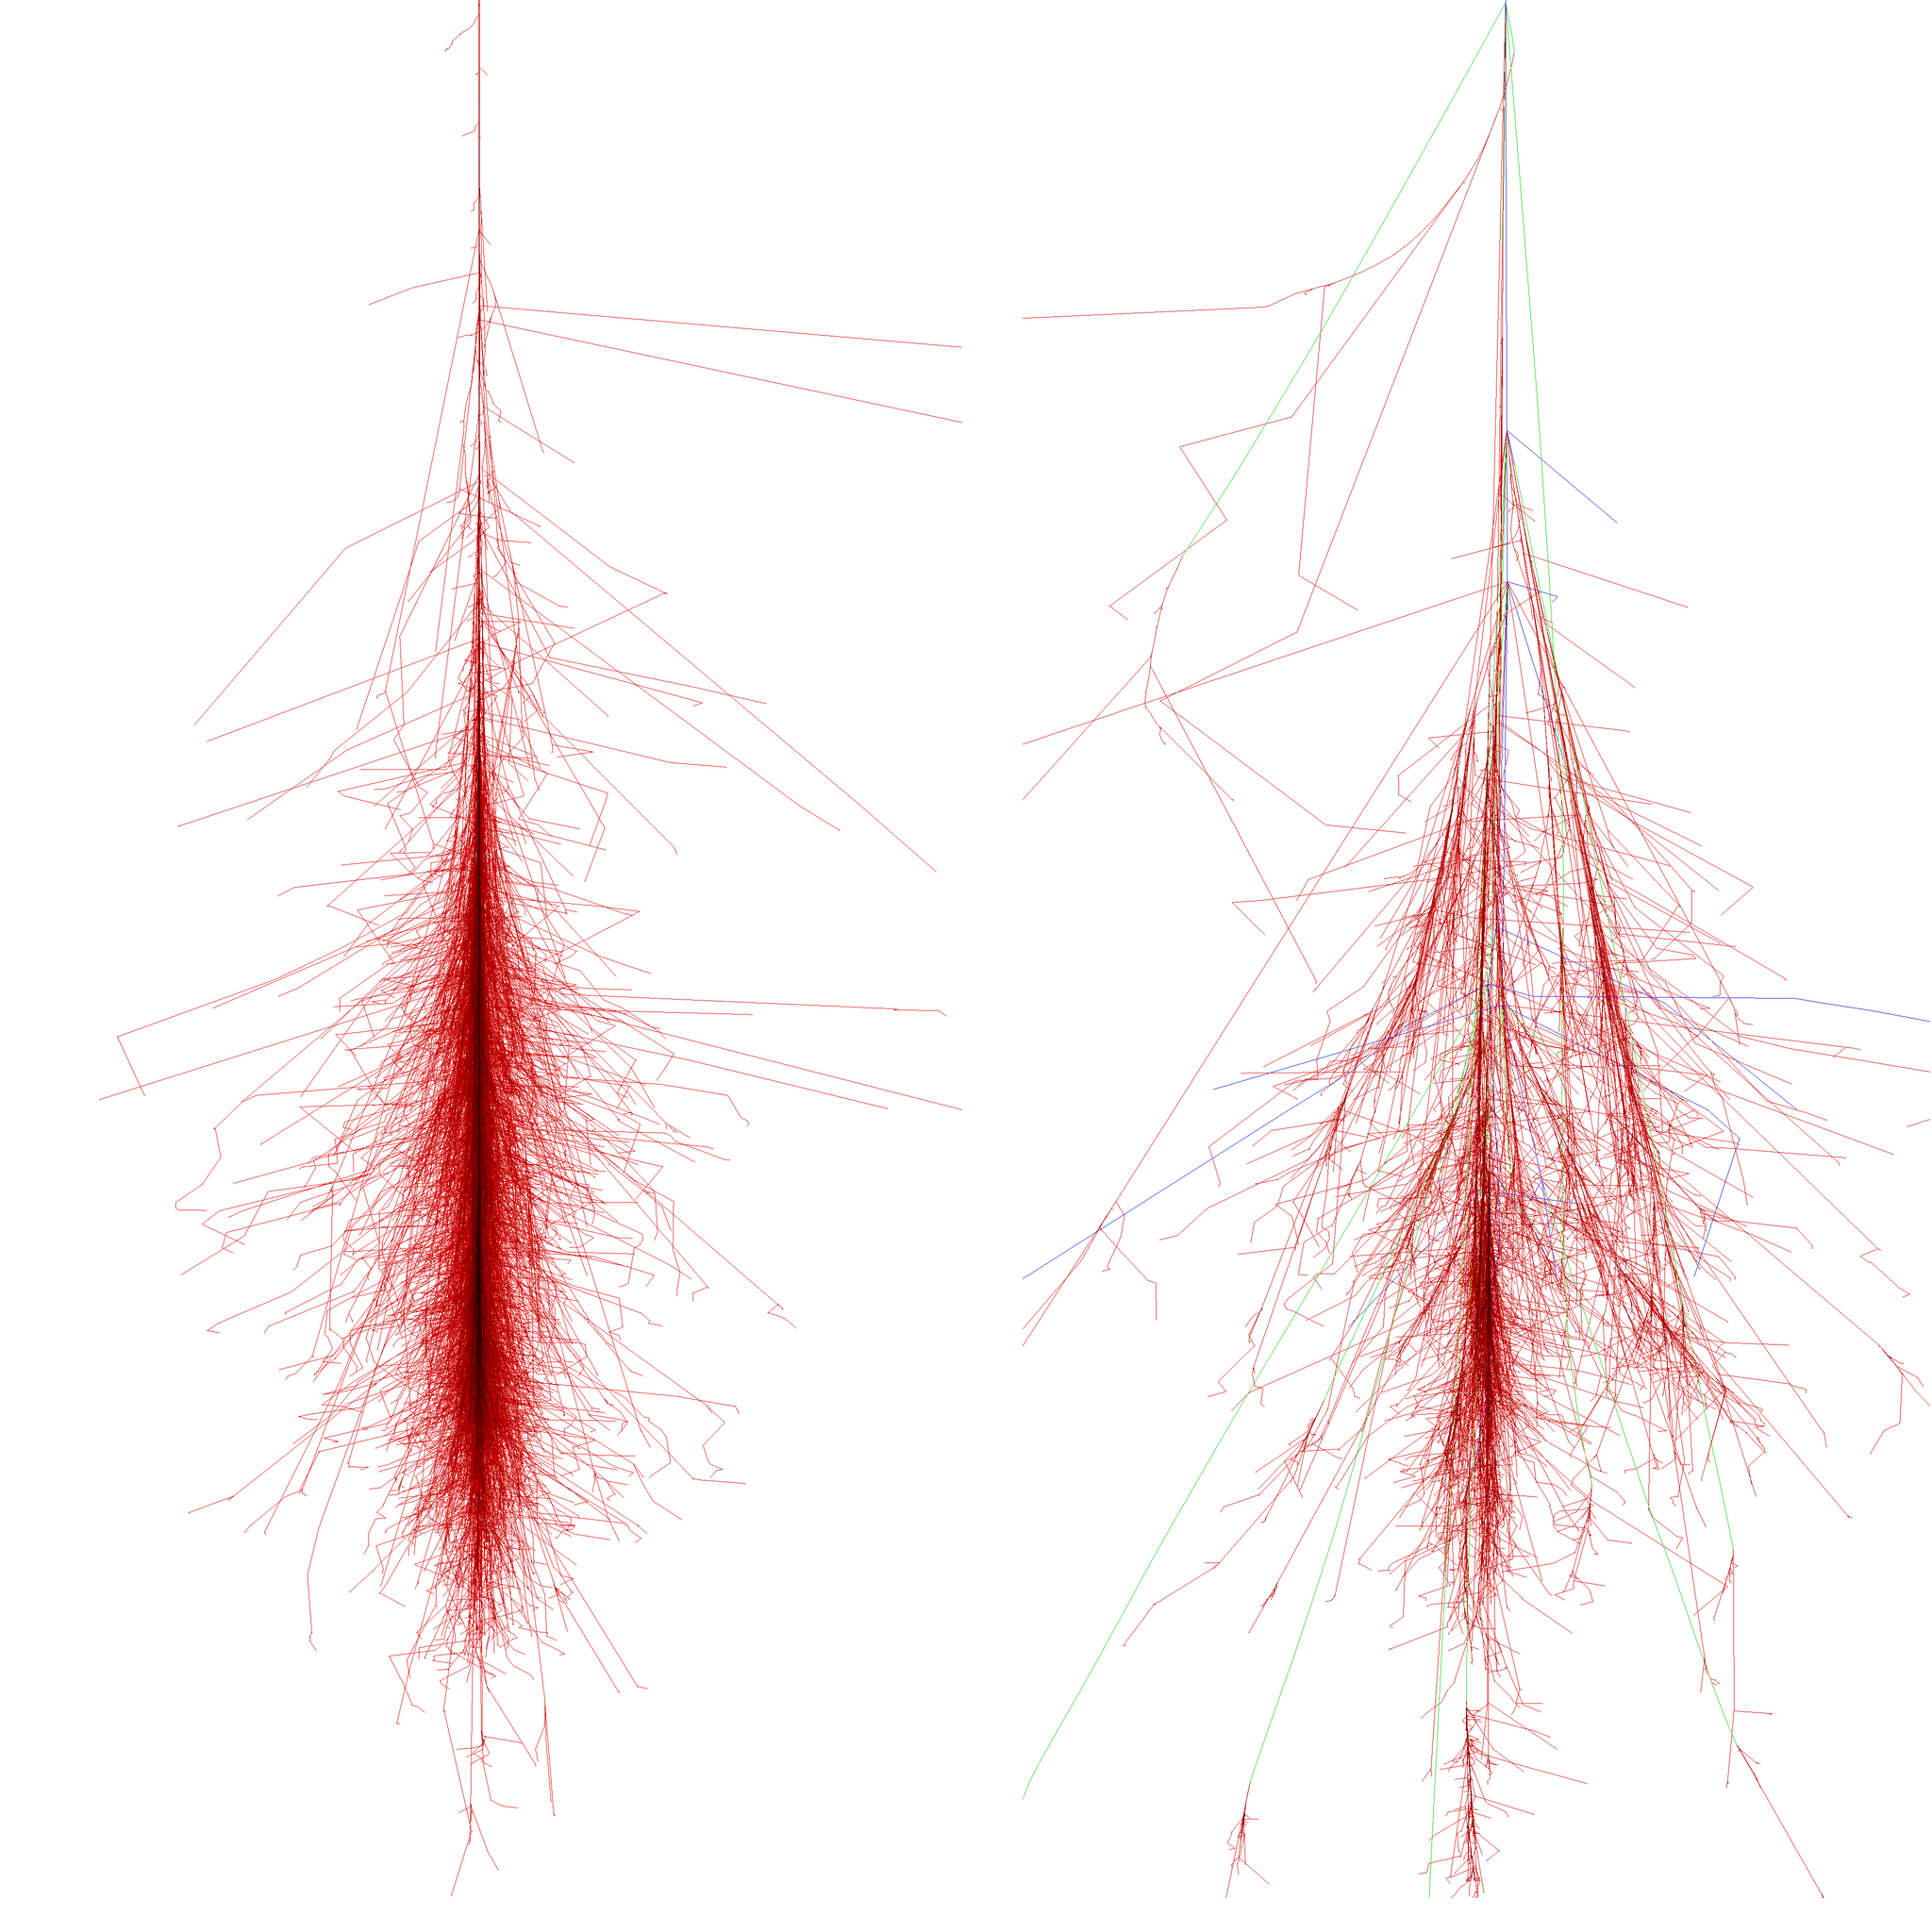
\includegraphics[width=\columnwidth]{figures/showers.png}
 
\caption{XZ plots of \textit{CORSIKA} simulations of particle tracks for $\mathrm{100\,GeV}$ photon (left) and proton (right) events. $\mathrm{e^+,e^-}$ and $\gamma$-rays are shown in red, $\mathrm{\mu^+\ and\ \mu^-}$ in green, and hadrons in blue. Note the wider, less concentrated proton shower which contains muons and hadrons that the $\gamma$-ray shower lacks (taken from \cite{corskplot}).}
\label{fig:image2}
\end{center}
\end{figure}
\subsection{Electron Air Showers}

In addition to the charged hadrons previously discussed, electrons can also be a significant source of background at low TeV energies. This is as they are difficult to distinguish from $\gamma$-rays and undergo similar interactions. There are two small differences between electron and $\gamma$-induced air showers. The first is the process by which the primary particles interact on hitting the atmosphere, a primary $\gamma$-ray will typically loose all its energy in a single pair production event. A primary electron of the same initial energy can loose energy via production of numerous lower-energy Bremsstrahlung photons which can create electromagnetic sub-showers. This can create a relatively greater number of Cherenkov photons at higher altitudes for electron-induced showers. The other small difference between electron and $\gamma$-ray induced showers is the average altitudes at which they first interact \cite{Sitarek1i}, which is due to the radiative length of an electron being smaller than the pair production length of a $\gamma$-ray. As a result, a primary cosmic-ray electron of the same energy as a primary $\gamma$-ray will begin interacting higher in the atmosphere. This results in a higher-altitude shower maximum \cite{lypova}. 

\subsection{Night Sky Background}
Not all of the background observed by an IACT can be attributed to EAS from charged particles. Night Sky Background (NSB) is the light detected in IACT camera images that is not Cherenkov light. In general, it is highly complex and poorly understood. It consists of photons from a variety of sources (including, but not limited to)

\begin{itemize}
    \item Atmospheric air glow emission lines, particularly from atomic oxygen, hydroxide and sodium.
    \item Moonlight.
    \item Starlight.
    \item Light from planes and satellites.
    \item Zodiacal light, along with diffuse galactic light and extragalactic background light (though these contributions are small) \cite{nsbref}.
    \item Light pollution from population centres.
\end{itemize}

Historically, analytic studies of NSB have been limited, as standard EAS and IACT simulation packages do not attempt to model NSB in a realistic way (for entirely legitimate reasons of computational cost). Most previous work on NSB has focused on direct observations with photomultipliers \cite{BandE}. We investigate the potential for advanced NSB modelling and how it might aid deep learning analysis in Chapter \ref{ch:5-CHECNSB}.

\section{Standard IACT Stages of Event Analysis}\label{app:imaging}
Now that we have established the basics of IACT operation, we turn to describing the stages that transform IACT event images into high-level astrophysical data.
\subsection{Trigger Selection}

Trigger selection is the first step in an IACT analysis chain. It is a feature of an IACT array designed to automatically reject events with a low probability of being astrophysical $\gamma$-rays in the readouts of the camera. CHEC-S, for example, only reads out the camera photomultipliers if two adjacent superpixels (blocks of four adjacent pixels) passes a comparator check. Being a significant influence on the results in Chapter \ref{ch:4-VERITASRealData}, the VERITAS trigger is slightly more complex. It consists of a single pixel trigger which acts on individual pixels (and includes timing analysis), a camera level trigger which works on the pattern and relative timing of the single pixel triggers, and an array trigger which requires that more than two telescopes are triggered in order such that an event is stored to disk \cite{veritastrigger}. This array-level trigger in particular significantly reduces the number of false triggers associated with muons passing through the instrument and telescope optics, as it is unlikely a single cosmic ray muon will generate sufficient Cherenkov light to trigger a second VERITAS telescope a few tens of meters away. 

\subsection{Pedestal Subtraction/Calibration}

After trigger selection, the next step is low level calibration. Electronic noise present in IACT camera data needs to be removed. For this purpose, measurements of the camera noise are taken when the camera is shut off from the outside environment with the shutter closed (similar to dark framing for optical astronomy). These measured pedestals are then subtracted from the observed live data. Flat-fielding of Cherenkov cameras is also necessary; it is typically performed by firing blue LED flasher units with known intensity profiles at the cameras.

\subsection{Charge Integration}

Once the raw data has been calibrated, the total number of photons collected by the photomultiplier from the EAS must be measured. Charge integration is the process of taking a calibrated PMT trace and extracting the number of photoelectrons. Various schemes exist for performing this operation, CHEC/SSTCAM relies on a cross-correlation template fitting model developed by J. Watson \cite{jasonthesis}.

\subsection{Tailcut Cleaning}

The next step in a conventional IACT analysis is tailcut cleaning. Before conventional IACT event reconstruction and classification, the sensitivity of these tasks to features in images from NSB requires that the images from the Cherenkov cameras are cleaned. The standard method of doing this is tailcut cleaning with two thresholds, whereby a pixel is only included in the analysis if the number of photoelectrons in the pixel exceeds a given threshold, or if it is the neighbour of such a pixel and also has a greater number of photoelectrons than a (typically lower) second threshold \cite{hegratailcut}. These thresholds require optimisation to achieve a desired event rate, and the implementations of this procedure vary by instrument (see for example \cite{Benbow} \cite{magictailcut} \cite{magictime}). Alternatively methods based upon wavelet image cleaning have been proposed \cite{wavelet}, but these are far more rarely used in practice. One of the aims of deep-learning-based image analyses that we explore in Chapters \ref{ch:3-TimingInfo} and \ref{ch:4-VERITASRealData} is to avoid this tailcut cleaning step, as some light from the Cherenkov shower itself is sometimes lost, however previous attempts at performing deep learning without requiring this step have failed when the event classifier or reconstruction method is exposed to real observations. 

\subsection{Hillas-Parameter-Based Techniques for Event Classification}

\begin{figure}[ht] 
        % read manual to see what [ht] means and for other possible options
        \centering 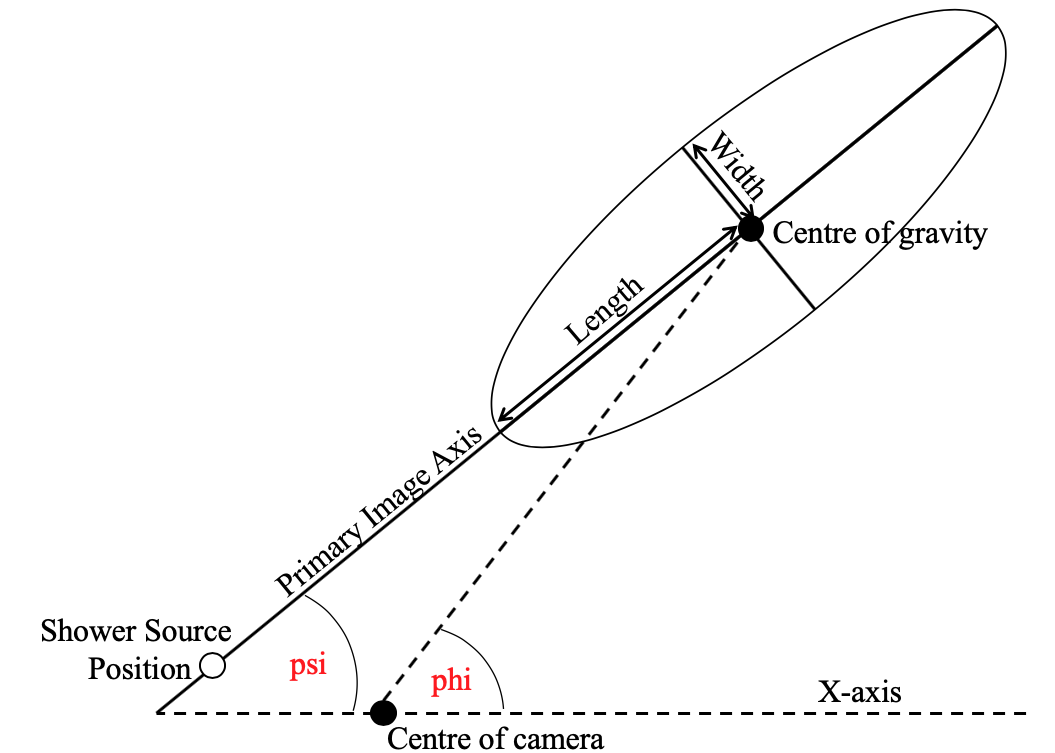
\includegraphics[width=\columnwidth]{figures/hillas.png}
        % note that in above figure file name, "sr_setup",
        % the file extension is missing. LaTeX is smart enough to find
        % apropriate one (i.e. pdf, png, etc.)
        % You can add this extention yourself as it seen below
        % both notations are correct but above has more flexibility
        %\includegraphics[width=1.0\columnwidth]{sr_setup.pdf}
        \caption{
                \label{fig:hillas} % spaces are big no-no withing labels
                % things like fig: are optional in the label but it helps
                % to orient yourself when you have multiple figures,
                % equations and tables
                The definition of Hillas parameters, taken from \cite{ctapipe}.
        }
\end{figure}
Hillas Parameters form the basis of the methods for event discrimination in the current generation of IACTs, and were instrumental in obtaining the first reliable gamma-ray source detection of the Crab nebula from the ground \cite{whipple} (several detections of astronomical objects were claimed before this but have since been disproved \cite{hintonicrc30} \cite{paulathesis}). They are obtained \cite{tomthesis} \cite{weekestev} from the second moments of an IACT camera image (constructed from the total integrated charge for each photomultiplier pixel), defined as 
\begin{align*}
\langle x^2 \rangle = \frac{\sum_i I_i x_i^2}{\sum_i I_i} && \langle y^2 \rangle = \frac{\sum_i I_i y_i^2}{\sum_i I_i}
\end{align*}
where $x_i$ and $y_i$ are the pixel co-ordinates and $I_i$ the associated pixel intensity. From these and the expectation values of $x$ and $y$ one can construct the variance and covariance
\begin{align*}
\sigma_x^2=\langle x^2 \rangle - \langle x \rangle^2&&\sigma_y^2=\langle y^2 \rangle - \langle y \rangle^2&&\sigma_{xy}=\langle xy \rangle - \langle x \rangle\langle y \rangle
\end{align*}
and define the following quantities
\begin{align*}
d=\sigma_x^2-\sigma_y^2&&a=(d+\sqrt{d^2+4\sigma_{xy}^2})/2\sigma_{xy}.
\end{align*}
The Hillas Parameters relevant for event classification are the width and length of the ellipse which characterize the transverse development of the shower and are defined by
\begin{align*}
W=\sqrt{\frac{\sigma_y^2+a^2\sigma_x^2+2a\sigma_{xy}}{1+a^2}}&&L=\sqrt{\frac{\sigma_x^2+a^2\sigma_y^2+2a\sigma_{xy}}{1+a^2}}.
\end{align*}
In order to take into account information from all of the telescopes in the array, these parameters must be combined into the Mean Reduced Scaled Width and Length (MRSW/MRSL), defined by a sum over all telescopes such that
\begin{align*}
SW&=\frac{W-\langle W \rangle}{\sigma_W}   &    SL&=\frac{L-\langle L \rangle}{\sigma_L}\\
\\ MRSW&=\frac{1}{\sum \omega}\sum SW\cdot \omega & MRSL&=\frac{1}{\sum \omega}\sum SL\cdot \omega
\end{align*}
where $\sigma_W$ is the spread of the expected width which must be obtained from Monte-Carlo generated lookup tables and $\omega=\langle W \rangle^2/\sigma_W^2$ is a weighting factor to take into account these tables' accuracy.

Initially Hillas Parameters were simply used to perform data cuts to separate hadronic showers from $\gamma$-ray induced showers based on their differing morphology. A combination of trigger selection and simple parameter-based cuts can reduce the signal to background ratio to $\sim$1:1 for a bright source like the Crab Nebula using a current generation instrument like H.E.S.S. \cite{Berge07}. In recent years, more sophisticated decision-tree-based methods such as Boosted Decision Trees (BDTs) or Random Forests (RFs),  (taking the MRSL, MRSW, total integrated charge and other parameters derived from Monte-Carlo lookup tables) eventually became the preferred methods for incident particle classification \cite{hessbdt}. These are essentially a sophisticated method of performing Hillas Parameter Cuts. For $\gamma$-hadron separation, H.E.S.S. \cite{hessbdt} and VERITAS \cite{evdisp} typically use BDTs whereas MAGIC normally uses RFs. An example of a binary tree structure used for IACT event classification can be seen in Figure \ref{fig:bdtstruct}. In this, events are classified as either Signal (S) or Background (B) by the tree based on whether at each node on the tree the parameters $m_{i,j}$ for a given event are larger than the weights $M^c=(m^c_j,...)$. During training, these weights are optimised to produce the desired results for the training data. The ultimate event classification is not performed by one tree, but by  an ensemble of trees in order to improve performance (the same is true for RF methods). BDTs iteratively improve tree performance by increasing the weighting for events that we misclassified by the previous tree in all subsequent trees. In the common Adaboost BDT optimisation algorithm, this weighting factor $\alpha$ is given by 
\begin{equation}
    \alpha=\frac{1-\mathrm{err}}{\mathrm{err}}
\end{equation}
where $\mathrm{err}$ is the fraction of misclassified events in all leaves (endpoints in Figure \ref{fig:bdtstruct}) of the decision tree \cite{hessbdt}. In RFs, a similar effect as achieved by randomly selecting a subset of input features at each node’s splitting point. One of the greatest advantages of decision-tree-based methods is that it is comparatively trivial to determine features in the input data that contributed to a classification; typically for IACT data the most important feature is the MSCW, but at energies below $\mathrm{100\,GeV}$ estimation of $X_{Max}$ can be important \cite{hessbdt}. These feature importances are not as trivial to obtain for the deep learning methods we will encounter in later chapters. BDTs and RFs can also be used to perform directional and energy regression for an event; for further technical details regarding the application of BDTs and RFs to IACT data see \cite{Sitarek1i} \cite{magictime} \cite{hessbdt} \cite{supermagictime}.

These techniques based on Hillas parameterisation don't however take advantage of the full camera image of the EAS, and as such, subtle details (such as hadronic `halos' \cite{model++}) in the images are not taken into account. This becomes an issue at the sensitivity boundaries that CTA is aiming to considerably improve (particularly in the case of weak or very extended sources), as hadronic and electron induced showers at these energies can closely resemble those generated by $\gamma$-rays. This motivates us to investigate new analysis techniques for event discrimination in order to improve the IACT sensitivity, as even small improvements to $\gamma$/hadron separation can translate into a significant increase in performance.

\begin{figure}[ht] 
        % read manual to see what [ht] means and for other possible options
        \centering 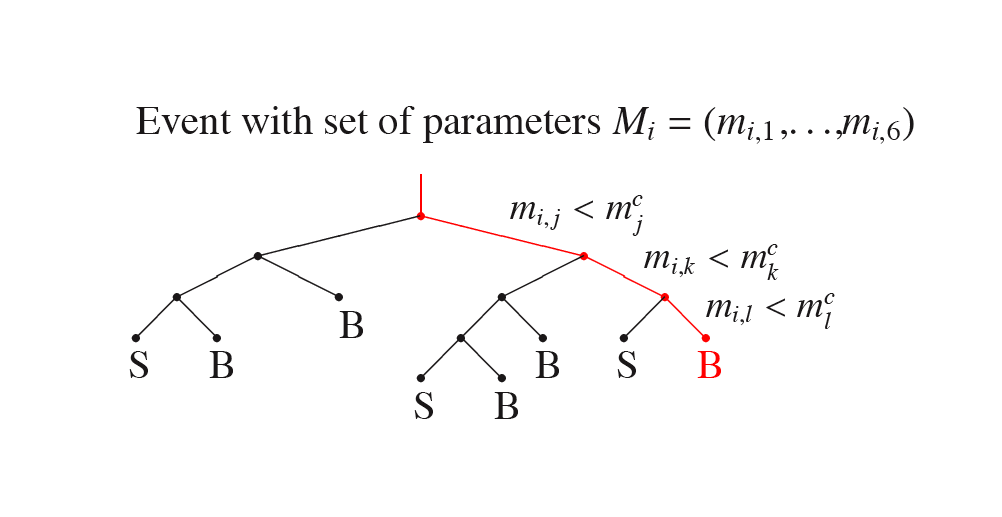
\includegraphics[width=\columnwidth]{figures/forest_picture.png}
        % note that in above figure file name, "sr_setup",
        % the file extension is missing. LaTeX is smart enough to find
        % apropriate one (i.e. pdf, png, etc.)
        % You can add this extention yourself as it seen below
        % both notations are correct but above has more flexibility
        %\includegraphics[width=1.0\columnwidth]{sr_setup.pdf}
        \caption{
                \label{fig:bdtstruct} % spaces are big no-no withing labels
                % things like fig: are optional in the label but it helps
                % to orient yourself when you have multiple figures,
                % equations and tables
                An example of a BDT, taken from \cite{hessbdt}.
        }
\end{figure}

\subsection{Event Selection Cuts and Run Selection}

IACT observations are normally conducted in runs, where the IACT array tracks and observes a single source. The duration of these runs varies, but most IACT observatories use between 20 and 30 minutes. This is long enough to obtain a sufficient number of events to accurately model the background, but short enough to ensure that the observation conditions are roughly constant.

Most IACT astronomical analyses begin with Hillas parameter cuts on the data to remove obviously hadronic events (with very high MRSW) and events far from the desired source (so-called theta-squared cuts). It is also common to remove runs or events from an IACT analysis for a variety of reasons. The data from a run may be low quality due to poor weather conditions, hardware or tracking issues or large zenith angle (at which simulation accuracy drops due to the complexity of modelling the atmosphere correctly). Most IACT analyses use multiple runs per source, though the work in Chapter \ref{ch:4-VERITASRealData} considers only a single VERITAS run as we attempt to match the data more closely with simulations.

\subsection{ON/OFF Region and Reflected Region Analysis}
So far we have focused on Cherenkov camera based background rejection, however this only reduces the signal to background rate (by around a factor of 100) to $\sim$1:1 for bright sources. As such, there is a need for a higher level background rejection method, similar to aperture photometry in optical astronomy. The simplest method possible is to take one ON region and one OFF region at the same right ascension but differing declination and use this to compute the $\gamma$-ray excess. The disadvantage of this is the loss of time on source. An alternative developed by the Whipple observatory is so called `Wobble Mode', where the telescope wobbles around the source in declination, allowing for more time on source. However, this is complicated by two factors, the comparatively poor angular resolution of IACTs, and the significant extension of some sources such as the supernova remnant RXJ 1713.7-3946. As such, the HEGRA collaboration \cite{HEGRA} developed so called reflected-region analysis, where multiple non-overlapping OFF regions (at different distances from the ON region but of the same angular size) are used. This allows for better statistics compared to a singular OFF region and allows for measurement of a potentially non-uniform night sky background across the field. This is the technique we use in Chapter \ref{ch:4-VERITASRealData}. However, such methods can run into difficulties for very extended objects such as Geminga, as the size of the source emission region might exceed the size of the FoV \cite{geminga}. In such scenarios a `FoV' background model, which models the radial acceptance of the IACT system can be used. The technical details of this are beyond the scope of this thesis; for more detail we refer the reader to \cite{Berge07} and \cite{geminga}. 

\subsection{Pointing Corrections}
Also necessary for reliable IACT operation is pointing calibration, as the size of the telescopes means they can bend slightly \cite{veritasstat}. This is typically performed by reconstructing the positions of stars using CCDs attached to the telescope structure, though SSTCAM has a slow signal chain to perform this (we explore the consequences of this in Chapter \ref{ch:5-CHECNSB}). This allows for positions of $\gamma$-ray sources to be reconstructed to within 2-3'; this can be important, especially for sources with extended morphology \cite{cena} \cite{rxjcta}.

\subsection{CTA Data Analysis Levels}

The proposed CTA analysis pipeline consists of a number of data analysis levels. Data processors exist to transform data at each level into the next. Only some of these levels are relevant for deep learning analyses. The current CTA data structure consists of \cite{jasonthesis}:
\begin{itemize}
    \item \textbf{r0 data}, which is the uncalibrated raw data generated by the Cherenkov camera.
    \item \textbf{r1 data}, which is online, calibrated camera data, calibrated using a scheme specific to the camera.
    \item \textbf{dl0 data}, which is calibrated waveform data along with event metadata, and is zero suppressed to save bandwidth and storage space.
    \item \textbf{dl1 data}, which consists of extracted charge and peak time information extracted from the calibrated waveforms, as well as Hillas parameters extracted from them.
    \item \textbf{dl2 data}, at this stage the telescope multiplicity is dropped and the overall events are characterised (based on their Hillas parameters extracted during the dl1 stage) into shower parameters including energy, direction, and source particle
    \item \textbf{dl3 data}, at this stage the dl2 events are sorted into sets of (for example) $\gamma$-ray candidates. This also includes any relevant instrument response data needed for higher level analysis.
    \item \textbf{dl4 data}, which consists of fully processed event lists, ready for high level astronomical analysis.
    \item \textbf{dl5 data}, which consists of high level analysis data products produced from astronomical analysis, such as the CTA galactic plane survey.
\end{itemize}

The CTA analysis chain will therefore reduce the raw amount of data from the telescopes from Petabytes to data scales tractable with a laptop.

\section{Alternatives to Hillas-Parameter-Based Techniques}
In this section we briefly consider the existing alternatives to Hillas analysis for IACT event classification and reconstruction.
\subsection{Template Analyses and Model++}
Template analyses \cite{model++} \cite{cat} \cite{3danalysis}  \cite{impact} form the current main alternative to Hillas parameterisation. They rely on the generation of a library of template IACT images. The images from the IACTs are then compared to the templates via a pixel-by-pixel minimisation process, such that the template most resembling the IACT image can be found and thus the shower properties inferred. In particular, the H.E.S.S. Model++ analysis chain uses chi-squared fitting against semi-analytic models of $\gamma$-ray showers as a background rejection method \cite{model++}. As Model++ is not open-source, it is not currently being considered as an analysis method for CTA, and its efficacy in the SST energy range has also not been tested. At the time of writing there is not a major effort within CTA to recreate it.

\subsection{ImPACT}
The most widely used template analysis is using the \textit{Image Pixelwise fit for Atmospheric Cherenkov Telescopes} (ImPACT) code \cite{impact}. This works by comparing the shower images to interpolated templates generated using Monte-Carlo simulations. ImPACT was developed for the (previously unprecedentedly large) H.E.S.S. CT5 telescope as Hillas parameter based techniques are known to be unreliable at photon energies lower than $50 \rm{Ge}V$.  The reconstructed event parameters are the combination of shower parameters for the template which minimizes the total negative log likelihood $\ln\mathcal{L}=\sum_{pixel,i}-2\ln{P(s_i|\mu,\sigma_p,\sigma_y)}$(maximizes the likelihood) over every pixel in the camera for every telescope in the array, where
\begin{equation}
P(s_i|\mu,\sigma_p,\sigma_y)=\sum_n \frac{\mu^n e^{-\mu}}{n!\sqrt{2\pi (\sigma_p^2+n\sigma_{\gamma}^2)}} \exp \left(-\frac{(s-n)^2}{2(\sigma_p^2 + n \sigma_{\gamma}^2)} \right)
\end{equation}
$n$ is the photoelectron number, $\sigma_p$ is the pedestal width (the width of the charge distribution under pure noise), $\sigma_{\gamma}$ represents the photomultiplier resolution, $s$ is the number of signal photoelectrons detected and $\mu$ is the predicted number of photoelectrons from the template. In practice, ImPACT is only used for directional and energy reconstruction in H.E.S.S. due to concerns about its sensitivity to NSB photons (a problem similar to the real observations problem experienced by Convolutional Neural Network (CNN)-type methods that we will explore in Chapters \ref{ch:2-CNNs}, \ref{ch:3-TimingInfo} and \ref{ch:4-VERITASRealData}). The H.E.S.S. ImPACT chain uses a BDT based on Hillas Parameters for $\gamma$/hadron separation. The ability of ImPACT to utilise stereoscopic sets of complete IACT images can significantly improve directional reconstruction compared to Hillas-parameter-based methods, especially at low energies \cite{impact}.

The difficulty in using ImPACT for CTA is the requirement of having a sufficient number of template simulations to cope with every possible type of event with a given energy and incident direction for a large number of telescopes, and the computational cost of searching through those simulations to find the optimal event parameters. That said, there is an open-source implementation of ImPACT available within \textit{ctapipe}.

\section{\textit{ctapipe} and the Prototype CTA Analysis Chain}

CTA is an instrument that is currently in the development phase, and this is true both of the instruments and the analysis pipelines that go with them. For much of the writing of this thesis a full, pythonic analysis pipeline for CTA did not exist, and CTA analyses were a complex mixture of modern code and software written for previous instruments. Additionally, a detailed, complex Monte-Carlo validation procedure was underway relating to the simulated data for even the prototype cameras.

\textit{ctapipe} is a python-based tool developed as an open-source prototype (which follows modern code practices for version control and code development) for the low-level analysis of CTA data. It is now recognised as a critical tool for CTA pipeline development, and is used in much of the analysis in this thesis. It provides tools to both handle \textit{CORSIKA}/\textit{sim\_telarray} simulations, perform data calibration and charge extraction, and to extract Hillas and muon ring parameters for events. It also contains \textit{astropy} based tools to compute camera pixel positions on sky, needed for the NSB work we present in Chapter \ref{ch:5-CHECNSB}. \textit{ctapipe} can even be used to analyze data from existing and historical IACT arrays; elements of our VERITAS work in Chapter \ref{ch:4-VERITASRealData} used reverse engineered code from ctapipe.

\textit{gammapy} and \textit{ctools} are the current open-source prototypes for high-level analysis (following similar development practice to \textit{ctapipe}); of these \textit{gammapy} has been selected as the high-level science tool for CTA. These allow one to generate source significance maps, lightcurves and spectra using IACT event lists. For simplicity, our \textit{VERITAS} work utilised the older, more stable \textit{Eventdisplay} tools for the work presented in Chapter \ref{ch:4-VERITASRealData}. But in time, high level data from all existing IACTs could be analysed with these new open-source packages.

\section{Methods and Environments of Astrophysical \ensuremath{\gamma}-ray Emission}
\subsection{Inverse Compton Scattering}

In this section we briefly discuss how and where astrophysical $\gamma$-rays are produced. The majority of astrophysical $\gamma$-rays are believed to be produced by Inverse-Compton (IC) scattering. IC scattering describes the process by which low energy photons are scattered by ultra-relativistic electrons, significantly increasing the energy of the photons. The so-called seed photon fields accelerated by the electrons vary; they can be a population of photons produced through synchrotron emission that are then hit by the high energy electrons that emitted them (so-called synchrotron self-Compton emission), can be the result of starlight, or originate from the Cosmic Microwave Background (CMB). In the rest frame of the electron, the ratio of final photon energy over initial energy is given by
\begin{equation}
    \frac{E_f}{E_i}=\gamma (1+\beta \cos(\theta))
\end{equation}
where $\gamma$ is the Lorentz factor of the electrons and $\theta$ is the deflection angle. Transferring to the observer frame this works out at around $\frac{E_f}{E_i}\sim \gamma^2$. Using this, combined with considerations of the energy density of the photon field ($u_{rad}$ in the observer frame), it can be shown \cite{longair} that the energy loss rate from a relativistic electron travelling at speed $\beta$ (where $\beta=\frac{\mathrm{v}}{\mathrm{c}}$ due to IC scattering is

\begin{equation}
    \left(\frac{dE}{dt}\right)_{\mathrm{IC}}=\frac{4}{3}\sigma_T c u_{\mathrm{rad}}\left(\beta^2\right)
\end{equation}

This results in the spectral emissivity from IC scattering of an isotropic photon field of single photon frequency $\nu_0$ by a power law distribution of electrons being given by 
\begin{equation}
    I(\nu)d\nu=\frac{3\sigma_TcvN(\nu_0)}{16\gamma^4\nu_0^2}\left(2c\ln\left(\frac{\nu}{4\gamma^2\nu_0}\right)+\nu+4\gamma^2\nu_0-\frac{\nu^2}{2\gamma^2\nu_0}\right)dv
\end{equation}
where $N(\nu_0)$ is the number density of photons, $\sigma_T$ is the Thompson cross section and $\nu$ is the frequency of the $\gamma$-rays \cite{blumenthal}.


\subsection{Hadronic Emission}
The second method of producing astrophysical $\gamma$-rays is through hadronic interactions. As we saw for EAS, proton-proton interactions can produce $\pi^0$ particles which decay to a pair of $\gamma$-rays. Hadronic emission processes are challenging to discriminate from IC scattering in some sources, particularly supernova remnants \cite{rxjcta}. The recent detection of an astrophysical neutrino (IceCube-170922A) by IceCube that was coincident with a $\gamma$-ray flare of the blazar TXS 0506+056 suggests that some $\gamma$-rays from AGN are produced by hadronic processes \cite{TXS}. 

\subsection{Supernova Remnants and Pulsar Wind Nebulae}
Now that we have considered the physical mechanisms by which astrophysical $\gamma$-rays are produced, let us consider the environments where this production might occur. Given the innately high energies involved, supernova remnants are prime sources of galactic $\gamma$-ray emission. Supernova remnants are also suspected of being one of the galactic sources of the highest energy cosmic rays (so-called PeVatrons). Most notably the supernova remnant RXJ1713.7-3946 has been detected to be spatially extended by H.E.S.S.; CTA might help to understand the emission mechanisms present in this source \cite{rxjcta}. Pulsar Wind Nebulae (PWN, also known as Plerions) such as the Crab Nebula are another, older related class of $\gamma$-ray sources where a wind from a central pulsar interacts with the surrounding ejecta to produce high-energy emission \cite{magiccrab}. A certain fraction of these PWN are so-called TeV Halos, highly-evolved (believed to be older than 100 kyr) systems where the pulsar has passed through the ejecta (after receiving a kick) from the associated supernova remnant and is now accelerating electrons in a spatially isolated region \cite{tevhalo}. Geminga is a likely candidate for such a system \cite{geminga}.

\subsection{$\gamma$-ray Binaries}
$\gamma$-ray Binaries are similar to their X-Ray counterparts, where a compact object (such as a neutron star or black hole) accretes matter from a companion star. $\gamma$-ray binaries differ from X-Ray Binaries typically because of the comparatively high mass of the companion star (typically an O or B class giant), as well as their higher-energy emission. Very few of these sources have been detected by IACTs ($\sim$10 at the time of writing), and they are generally fairly poorly understood \cite{scienceCTA}, with it often being unclear if the accreting compact object is a neutron star or a black hole. CTA will likely help us discover more of these objects and increase our understanding of those that have already been detected.

\subsection{Active Galactic Nuclei}
AGN are known sources of GeV and TeV $\gamma$-rays, typically these are blazars (where the jet of the AGN directly points towards Earth). These blazars fall into two categories based on how energetic they are, these are known as BL LACs (for the low energy case) or Flat Spectrum Radio Quasars (FSRQs, for the high energy case). The characteristic double-peaked Spectral Energy Distribution (SED) of blazars is evidence for there being some synchrotron-self-Compton emission from these objects. Flares (unusual periods of bright emission) from AGN are also observed as a class of extragalactic $\gamma$-ray transient, see for example \cite{TXS}.

\subsection{Galactic and Extragalactic Transients}
GRBs are typically bright, but comparatively short lived in their $\gamma$-ray emission. They are believed to originate from neutron star collisions or core-collapse supernovae; differences in the redshift distributions of short-lived and long-lived GRBs is evidence to support this hypothesis \cite{longair}. GRBs have only recently been observed from the ground, partly due to the technical challenge of turning the instruments quickly enough to detect the prompt emission, but also due to the complex factors involved in background rejection and the fact that most GRBs do not have spectra extending into the TeV. This first detection of a both prompt emission from a GRB and lower-energy afterglow from the ground by MAGIC and H.E.S.S. in 2019 \cite{magicGRB}.

The first galactic transient detected by an IACT was the recurring Novae RS Ophiuchi by H.E.S.S. [H.E.S.S. Collaboration, in prep]. Emission from Novae is typically a result of a thermonuclear explosion of the surface of an accreting white dwarf, although the source of the TeV photons is potentially unclear. This detection was somewhat unexpected, but suggests CTA might be able to detect a greater population of galactic transient objects.

\subsection{Diffuse Emission}
Both galactic and extragalactic diffuse $\gamma$-ray emission are observered by IACTs. In the galactic case it is believed the majority of the emission results from hadronic emission due to collisions of cosmic rays with galactic gas \cite{extragamma}. The extragalactic case is less well understood \cite{extragamma}, with the majority of emission likely due to unresolved blazars, radio galaxies and star-forming galaxies, but some additional components may be due to dark matter annihilation or cosmic ray interactions \cite{extragamma}.

\section{The Key Science Projects of CTA}
Now that we have discussed the origin and production of $\gamma$-rays, we will briefly discuss the observing strategy for the scientific investigations of CTA. The CTA observing time not allocated to open observations or Target of Opportunity (ToO) observations will be dedicated to a number of Key Science Projects (KSPs). In this section we briefly explore the science potential for each of these missions.

\subsection{The Galactic Centre KSP}
CTA observations will be made of the central square degree of the Milky Way for 500 hours \cite{scienceCTA}, with a further 300 hours spent observing the region up to 10 degrees in galactic latitude. It is anticipated that this will be one of the first major campaigns for CTA due to its implications for other CTA surveys.
In particular, the galactic centre is considered one of the best places to search for evidence of dark matter annihilation, and these observations should be sufficient to obtain either a detection or an upper limit for many of the current best dark matter models \cite{scienceCTA}. Additionally, these observations hope to uncover the nature of the galactic centre $\gamma$-ray source, and to probe the nature of very high energy particle acceleration in the galactic centre (key to understanding the nature of the Fermi Bubbles). 

\subsection{The Galactic Plane Survey (GPS) and the Cosmic Ray PeVatron KSP}
Around 1800 total hours of observing time will be spent performing observations of the galactic plane, with a sensitivity of at least 4.2 mCrab \cite{scienceCTA} (an improvement of 5-20 times relative to current instruments). It is planned that this survey will lead to the discovery of new galactic sources of TeV $\gamma$-rays, including supernova remnants, $\gamma$-ray binaries and Pulsar Wind Nebulae. Additionally, it will provide new constraints for models of the galactic diffuse emission and source populations. 

It is anticipated that the maps generated by the GPS will be periodically made public, in order to maximize its multi-wavelength science potential.
Additionally, the PeVatron KSP aims to perform dedicated, deep observations of known $\gamma$-ray sources with particularly hard spectra (such as RX J1713.7-3946), and search for diffuse $\gamma$-ray emission around known Supernova Remnants in an attempt to understand the origins and acceleration methods of cosmic rays \cite{scienceCTA}.

\subsection{The Large Magellanic Cloud Survey and the Star Forming Systems KSP} Around 600 hours of CTA observation time will be spent on observing the Large Magellanic Cloud (LMC). In particular, the LMC is interesting at TeV energies due to its high rate of star formation; the LMC produces about one tenth of the number of stars as the Milky Way, but has only 2\% of the Milky Way's volume \cite{scienceCTA}.
As such, it contains a disproportionate number of supernova remnants (such as SN1987A) and pulsar wind nebulae.  These can be observed more easily in the LMC than in the Milky Way due to the absence of source confusion, interstellar absorption and line of sight crowding at the LMC's high galactic latitude \cite{scienceCTA}. Other observations of galactic star forming regions (for example Westerlund 1) are also planned as part of the star forming systems KSP, in order to investigate the link between star formation and particle acceleration.

\subsection{The Extra-Galactic Survey and the AGN KSP} One of the largest time allocations, the extra-galactic survey will cover 25\% of the sky down to 6 mCrab sensitivity \cite{scienceCTA}. It will aim to achieve an unbiased census of $\gamma$-ray AGN, observe fast-flaring sources and gamma-ray busts serendipitously, and measure the anisotropies in the electron cosmic ray spectrum. Key to this is CTA's ability to operate in a divergent pointing mode, where not all telescopes in the array are pointing at the same patch on the sky. 

An AGN KSP is also envisaged to perform long term monitoring of a select set of Active Galactic Nuclei, in order to understand how the different types of AGN are related, and how their particle and $\gamma$-ray acceleration mechanisms work \cite{scienceCTA}. By extension, these observations should also act as a probe of the intergalactic magnetic field and the extragalactic background light. The AGN KSP is also a means of performing tests of fundamental physics, and CTA should be able to place constraints on Lorentz Invariance Violation and the production of Axion-like particles through the monitoring of AGN. 

\subsection{The Transient KSP} Somewhat intertwined with the Extra-Galactic Survey, CTA will have the capability to respond to transient events from both internal and external triggers. These external triggers will be sent by Gravitational Wave, Neutrino, Radio, Optical, X-ray and $\gamma$-ray observatories around the world when they detect a transient object. Following such a trigger, CTA will immediately perform follow-up observations to help constrain the emitting object's nature \cite{scienceCTA}. Likewise notifications of transient events serendipitously detected by CTA will be sent to partner observatories.

\section{Thesis Structure}
The remainder of this thesis is structured into five chapters. In Chapter \ref{ch:2-CNNs}, we introduce deep learning methodologies, before exploring past and concurrent work on their applications for IACTs, and then introducing multiple problems with such applications that are currently unsolved. In Chapter \ref{ch:3-TimingInfo} we explore the previously unconsidered option of utilising photosensor timing information as a basis for a deep learning event classification method, utilising the advanced capability of waveform storage possible with SSTCAM. In Chapter \ref{ch:4-VERITASRealData}, we explore the difficulties in using charge-based deep learning classifiers with existing data from VERITAS, exploring in detail the complication of optimising deep learning classifiers and the complexities arising from not wishing to perform tailcut image cleaning. Chapter \ref{ch:5-CHECNSB} concerns a detailed study into the likely NSB conditions experienced by SSTCAM. Whilst NSB represents a significant challenge to deep learning event classification and reconstruction methods, the work within this chapter is largely self-contained. Finally in Chapter \ref{ch6-Conclusions} we investigate future prospects for analyses in these fields and conclude.